%% usenix_sec2027.tex
%% USENIX Security 2027 submission build.
%%
%% Format contract (checked by the HotCRP auto-format checker):
%%   - two-column, 10pt body font on 12pt leading
%%   - 7.0in x 9.0in text block (set by usenix.sty; do not override)
%%   - up to 13 pages of body text; references and appendices are unlimited
%%     in the initial submission
%%   - an "Open Science" appendix is mandatory at submission
%%   - an "Ethical Considerations" appendix is strongly recommended
%%
%% Do not change \textwidth, \textheight, \columnsep, font size, or leading.

\documentclass[letterpaper,twocolumn,10pt]{article}

% amsmath/amssymb/amsthm are loaded before usenix.sty so that hyperref
% (loaded inside usenix.sty) is initialised last.
\usepackage{amsmath}
\usepackage{amssymb}
\usepackage{amsthm}

\usepackage{usenix}

\usepackage{booktabs}
\usepackage{array}
\usepackage{graphicx}
\graphicspath{{figures/}}

% Ragged-right variant of p{} for the narrow table columns.  Justifying a
% 0.25\columnwidth cell opens inter-word gaps wide enough to read as column
% separators; this only changes alignment inside those cells.
\newcolumntype{L}[1]{>{\raggedright\arraybackslash}p{#1}}

% Captions at 9pt: allowed by USENIX (the 10pt/12pt requirement applies to
% body text) and standard practice in the proceedings.
\usepackage[font=small,labelfont=bf]{caption}

% article's default float parameters are much stricter than IEEEtran's and
% push floats to the end of the document.  These values keep floats near
% their first reference without changing the text block.
\setcounter{topnumber}{3}
\setcounter{bottomnumber}{2}
\setcounter{totalnumber}{5}
\setcounter{dbltopnumber}{3}
\renewcommand{\topfraction}{0.92}
\renewcommand{\bottomfraction}{0.7}
\renewcommand{\textfraction}{0.07}
\renewcommand{\floatpagefraction}{0.7}
\renewcommand{\dbltopfraction}{0.92}
\renewcommand{\dblfloatpagefraction}{0.7}

% Float and display separations are left at the class defaults.  The CFP
% requires page limits to be met through content alone, so no white space is
% recovered anywhere in this file.

% correct bad hyphenation here
\hyphenation{op-tical net-works semi-conduc-tor}

\newtheorem{definition}{Definition}
\newtheorem{theorem}{Theorem}
\newtheorem{lemma}{Lemma}
\newtheorem{proposition}{Proposition}

\begin{document}

% no date on USENIX titles
\date{}

% Title registered for USENIX Security '27 Cycle 1 (fixed at registration,
% 2026-08-18).  Earlier candidates, no longer usable: "Trained Behind a
% Shield, Unsafe Without It: Reward Poisoning at Runtime-Assurance Authority
% Transitions"; "Reward Poisoning at Runtime-Assurance Authority Transitions".
\title{\Large \bf A Release Test Is Not Runtime Authority:\\
  Evidence Reuse at Runtime-Assurance Authority Transitions}

% Anonymous submission: do not add author names, affiliations, funding
% acknowledgments, or self-identifying artifact URLs before acceptance.
\author{}

\maketitle

\begin{abstract}
A learning-enabled controller can adapt while runtime assurance retains action
authority, then release a raw policy after a finite check.  Such evidence is
tied to the checked subject, authority, and horizon.  In Safe-Control-Gym, a
clean cohort of 20 independently trained controllers supplied 480 accepted
snapshot--state pairs.  Permanent raw release failed on 10 pairs across five
training runs, whereas resident predictive authority failed on none.  A
bounded reward-record attacker widened this gap while satisfying calibrated
known-sign and scalar-envelope checks.  After 48 protected update batches, it
caused 46/116 failures under raw release and 34/116 under resident authority.
Paired accounting found 27 failures under both contracts, 19 only under raw
release, seven only under resident authority, and 63 under neither.  Every
resident failure followed a switch to the trusted baseline, with a median of
one further step to violation.  Thus, repeated raw-policy checks did not also
establish the safety of the baseline handoff.  Bootstrap-only poisoning also
increased retirement violations in two of three provenance-complete pairs of a
published lifecycle.  Trusted recomputation closes the reward channel, but
each controller receiving authority still requires evidence for its own
deployment contract.
\end{abstract}

\section{Introduction}

Runtime assurance is the standard way to let a controller learn without
letting it crash the plant.  A Simplex decision module, a runtime shield, or a
model-predictive safety filter holds action authority during adaptation: it
replaces unsafe policy proposals with actions from a trusted baseline, so
every transition collected while the policy trains satisfies the safety
certificate~\cite{seto_simplex_1998,alshiekh_shielding_2018,
wabersich_linear_mpsc_2018}.  Deployments do not keep that machinery forever.
Published lifecycles and ordinary engineering practice retire the protective
authority once commissioning succeeds and promote the raw policy snapshot to a
lower-latency control target, which removes permanent computation,
intervention, and dependence on a backup
service~\cite{carr_partial_shielding_2023,hsu_sim_lab_real_2023}.  A finite
release check --- a bounded-horizon prediction, a certified rollout, a
commissioning test --- authorizes that promotion.

We show that the release check does not transfer across the retirement it
authorizes.  Protection makes the executed composition safe; it does not make
the raw policy safe.  The same finite check is sound while it retains
authority and unsound once it is spent at release, because release changes the
subject being authorized, the authority enforcing the decision, and the
horizon over which the evidence must hold.  We call the underlying flaw
\emph{evidence reuse across an authority transition}: evidence collected
during protected adaptation is reused to authorize a different subject, under
a different authority, with different provenance, information, and horizon.

\begin{figure}[t]
\centering
\fbox{\begin{minipage}[c][1.74in][c]{0.92\columnwidth}
\centering
\textbf{Asynchronous learning-data plane}\\[0.25em]
reward record $\xrightarrow{\text{bounded write}}$ trusted updater
$\rightarrow$ raw candidate\\
$\hspace{3.0em}\rightarrow$ one-time check $\rightarrow$ snapshot export\\[0.35em]
\rule{0.88\columnwidth}{0.3pt}\\[-0.15em]
\textbf{High-integrity runtime-assurance plane}\\[0.25em]
authenticated state $\rightarrow$ predictor/selector $\rightarrow$ actuator\\
$\hspace{3.1em}\uparrow$ trusted baseline\\[0.35em]
resident after check: timely switch\\
authority removed: delayed failure
\end{minipage}}
\caption{Evaluated trust boundary.  The benchmark begins after bounded
reward-record access is obtained; it does not model the initial service
compromise.  Upstream provenance or recomputation removes this attack path,
whereas resident predictive authority contains its downstream physical
consequence.}
\label{fig:lifecycle-placeholder}
\end{figure}

The gap is measurable without an adversary.  In our controlled study,
snapshots that passed a five-step release check failed on 2 of 120
snapshot--state pairs once released raw, whereas the identical prediction
retained at runtime failed on none.  Residence alone is not the remedy: on a
disjoint cohort, a one-step resident kernel failed on 14 of 71 accepted pairs
and reached an empty kernel 41 times.  What separates these outcomes is
whether a check with enough lookahead to leave switching lead time keeps
authority at runtime.

An upstream adversary widens the gap rather than creating it.  While the
shield masks unsafe proposals, corrupted update data steers the learner
without producing a single physical violation, and the damage stays latent
until authority is removed: bounded reward-record edits raised the same
120-pair count from 2 to 27.  We call this \emph{shield-retirement poisoning}.
Its applicability is narrow by construction (Section~\ref{sec:threat}): where
the runtime plane can recompute reward from authenticated transitions, trusted
recomputation removes the channel outright, as our frozen integrity audit
confirms.  The contract gap survives that defense.

The attacker we evaluate is deliberately weak.  Operational technology (OT)
guidance separates runtime-control assets from the data-management services
and historians that exchange information across
zones~\cite{nist_ot_security_2023,mitre_data_historian}, and our threat model
begins after compromise of a reward-ingestion principal in that learning-data
plane.  This is an explicit split-trust precondition: the attacker may modify
bounded scalar reward records consumed by a policy-gradient updater, and
nothing else.  Authenticated runtime states, actions, learner code,
parameters, optimizer state, certificates, and deployment states remain
outside its write authority (Fig.~\ref{fig:lifecycle-placeholder}).

Existing mechanisms address neighboring problems.  Simplex and its neural and
barrier-based successors keep a decision module resident
\cite{seto_simplex_1998,phan_neural_simplex_2020,damare_bb_simplex_2025}.
Policy repair and safe projection constrain a learned policy before deployment
\cite{zhou_runtime_policy_repair_2020,lu_repair_preservation_2024,
chow_safe_policy_2021}.  Reward-poisoning work studies how adversarial
learning signals redirect updates, but not behind a shield.  None treats the
release decision itself as the object of study: the unresolved composition is
a transition in which evidence produced under retained authority is spent
once, at release, to authorize a raw policy that will run without it.

\subsection{Evidence and Contributions}

We separate the contract gap from the channel that widens it.  The controlled
Safe-Control-Gym study supplies the counts above under a five-step check that
accepted every candidate, and adds a locked horizon sweep placing the usable
lookahead between an insufficient one-step check and an over-conservative
twenty-step one.  The channel is not confined to our harness: Carr et al.'s
published workflow trains a policy behind a Storm belief-support shield and
later retires the shield's authority~\cite{carr_partial_shielding_2023}, and
adding bounded reward-record poisoning only during the protected bootstrap
increased raw-policy violations at retirement by factors of 3.6 and 1.6 in two
of three provenance-complete paired REINFORCE training runs.

Our contributions are:

\begin{itemize}
    \item We formalize release-time acceptance as an evidence tuple over
    subject, authority, provenance, information, and horizon, and show that a
    deployment must re-establish every component the authority transition
    changes.
    \item We measure the resulting gap without an adversary, separating
    one-time raw release from resident predictive authority, one-step
    filtering, and commit admission, and locating the lookahead at which a
    retained check is neither insufficient nor over-conservative.
    \item We instantiate one upstream channel that widens the gap ---
    bounded reward-record writes --- in the controlled study and in a
    third-party shield-retirement lifecycle, and report the integrity controls
    that close that channel while leaving the gap open.
    \item We characterize the attack's empirical boundary across systems,
    learners, integrity controls, and deployment contracts: high
    retirement-state disagreement excludes every observed positive outcome in
    the locked corpus, while low disagreement defines an opportunity region
    without guaranteeing success.
\end{itemize}

\section{Background and Problem Model}
\label{sec:model}

\subsection{Attacked Histories and Plausible States}

We consider a discrete-time cyber-physical system
\begin{equation}
    x_{t+1}=f(x_t,u_t,w_t), \qquad
    \widetilde y_t=h(x_t)+a_t,
\end{equation}
where $x_t$ is the physical state, $u_t$ is the control input,
$w_t\in\mathcal W$ is ordinary process uncertainty, and $a_t$ is a
false-data injection (FDI) signal on the measurement channel.  The controller
observes the attacked history
\begin{equation}
    h_t=(\widetilde y_{0:t},u_{0:t-1},\widetilde\ell_{0:t}),
\end{equation}
where $\widetilde\ell_t=\ell_t+b_t$ is a learning signal modified by
update-data corruption $b_t$.  The general model covers rewards, logs, and
auxiliary learning signals; the end-to-end experiments specialize this channel
to bounded scalar reward-record edits.  Sensor FDI creates uncertainty about
the physical state, whereas update-data corruption can redirect learning even
with trusted state observations.  Either channel can change the action map
produced from $h_t$.

Following severe sensor-attack safety work~\cite{tan_safety_2024}, an attacked
history may correspond to multiple physical states.  For an attack family
$\mathcal A$, define the plausible-state set
\begin{equation}
    X_{\mathcal A}(h_t)=\{x:\exists E\in\mathcal A,\; H_t(E)=h_t,\; x_t(E)=x\}.
\end{equation}
This set defines the state semantics of a certificate under strategic FDI: a
certificate evaluated only at a nominal estimate $\hat x(h_t)$ does not cover
another compatible state in $X_{\mathcal A}(h_t)$.

\subsection{Online-Updated Controllers and Certified Kernels}

The controller is a history-dependent policy $\pi_{\theta_t}$ that selects
$u_t=\pi_{\theta_t}(h_t)$ and updates according to
$\theta_{t+1}=U(\theta_t,h_t)$.  An update is \emph{nontrivial} when it
changes the controller's action map on a reachable or admissible history;
parameter changes that preserve the action map are behaviorally trivial.

Let $\Gamma$ denote an invariant-set, barrier, reachability, or runtime-shield
certificate.  At history $h$, the certificate induces actions that are valid
for every plausible state:
\begin{equation}
    K_\Gamma(h)=\{u\in\mathcal U: u \text{ satisfies } \Gamma \text{ for all } x\in X_{\mathcal A}(h)\}.
\end{equation}
We call $K_\Gamma(h)$ the \emph{certified kernel}.  Severe-attack safety
filters construct or act within such kernels for fixed controllers.  Online
learning additionally requires admission of the updated action map produced by
$U$.

\begin{definition}[Certified online learning]
A mechanism is a certified online learner at history $h$ if it accepts a
certificate for $\pi_{\theta_{t+1}}$, where
$\theta_{t+1}=U(\theta_t,h)$.  The accepted certificate asserts that the next
certified action is sound for every state in $X_{\mathcal A}(h)$.
\end{definition}

\begin{definition}[Finite-horizon check]
Let $\mathcal H_{\mathcal A}^{\tau}(h,\pi)$ denote the attacked histories
reachable within the next $\tau$ steps from $h$ under policy $\pi$.  A
finite-horizon check is sound for its declared horizon if acceptance implies
that $\pi(h')$ satisfies $\Gamma$ for every
$h'\in\mathcal H_{\mathcal A}^{\tau}(h,\pi)$ and every
$x\in X_{\mathcal A}(h')$.  It makes no claim about histories outside this
set.
\end{definition}

\begin{definition}[Sound lifecycle certificate]
A certificate accepted for $\pi_{\theta^+}$ at history $h$ over attack family
$\mathcal A$ is \emph{sound} when it asserts, for every attacked history $h'$
reachable after $h$ under $\pi_{\theta^+}$ and every $x\in X_{\mathcal A}(h')$,
that $\pi_{\theta^+}(h')$ satisfies $\Gamma$.  An acceptance rule is sound for
a contract when acceptance implies the safety property that contract requires.
\end{definition}

\begin{definition}[Learning-freeze frontier]
For a family of histories parameterized by attack strength or ambiguity
radius, the learning-freeze frontier is the boundary at which
$K_\Gamma(h)$ becomes empty, the candidate updated action leaves
$K_\Gamma(h)$, or the candidate parameter leaves the corresponding certified
set $\Theta_\Gamma(h)$. Beyond this boundary, a sound certified learner must
reject the certificate, freeze the update, or obtain extra trusted state
information.
\end{definition}

\subsection{Assurance-Contract Failure Modes}
\label{sec:lifecycle-attacks}

Four failure modes arise at different points in the assurance lifecycle, and
three of them are already recognized.  \emph{Nominal-state certification}
evaluates the certificate at an estimate $\hat x(h)$, so under FDI an accepted
action may be unsafe for another state in $X_{\mathcal A}(h)$; severe-attack
safety filters address it.  \emph{Action-only filtering} projects the applied
action into $K_\Gamma(h)$ but leaves the updated action map a separate object,
so the certificate can cover the actuator channel while
$\pi_{\theta_{t+1}}(h)\notin K_\Gamma(h)$.  \emph{Uncertified learning after
rejection} occurs when an empty kernel forces a fail-safe action while an
update computed from the same attacked history proceeds anyway.

The fourth mode is the subject of this paper.  Under \emph{protected
adaptation with unsafe deployment}, an adaptation shield keeps every
data-collection transition safe.  Safety of those executed transitions does
not establish the behavior of the unfiltered raw policy that will later act
alone.  Raw release therefore requires evidence for the subject receiving
action authority.  Corrupted reward records are not needed to reach this mode;
they widen it by steering the trusted update rule toward a raw policy that
fails after retirement while protected execution remains safe.

These modes require separate metrics: accepted certificates whose applied
action is unsafe for some plausible state, accepted certificates for which the
updated raw policy leaves the kernel, and nontrivial updates after certificate
rejection.  End-to-end studies add delayed deployment violations, admission
coverage, paired clean/poison outcomes, update fraction, intervention, reward,
and certificate runtime.  Useful learning additionally requires paired task
improvement over always-freeze.

\section{Threat Model}
\label{sec:threat}

\subsection{System Roles and Deployment Contracts}

The defender deploys an online-updated controller $\pi_{\theta_t}$ and a
certificate mechanism; a severe-attack-aware estimator or filter returns a
plausible-state set $X_{\mathcal A}(h_t)$ and certified action kernel
$K_\Gamma(h_t)$.  A trusted state anchor, integrity-protected fallback
controller, or external fail-safe may also be available, but each is an explicit architectural
assumption and cost.
Unless a formal safety result is stated, \emph{trusted} and
\emph{integrity-protected} mean outside the attacker's write authority; they do
not mean that a controller or handoff is verified safe.

The evaluation instantiates four contracts.  \emph{Permanent raw release}
removes runtime authority after a one-time five-step raw-policy test: protected
commissioning is followed by snapshot export and promotion to a lower-latency
control target, which avoids permanent computation, intervention, and
dependence on a backup service.  \emph{Commit admission} certifies a candidate
snapshot on a declared state set and horizon before raw release.
The \emph{raw-policy lookahead switcher} repeats the same check online and can
transfer control to an integrity-protected LQR fallback.  The check supplies
evidence about the raw policy, not about LQR recovery from the handoff state;
the latter is a separate handoff obligation.  The \emph{one-step action
filter} applies a current-state action filter and serves as a negative
control.  A sound filter that remains online instead certifies the composition
$F\circ\pi_{\theta^+}$.  Each name denotes a distinct evidence scope and
authority contract, and Section~\ref{sec:study} measures their tradeoffs;
Appendix~\ref{sec:appendix-delta} gives a contract taxonomy.

\subsection{Split-Trust Learning Pipeline}

The split-trust model separates a high-integrity runtime-assurance plane
from an asynchronous learning-data plane.  The runtime plane owns the
authenticated plant state, action selector, actuator interface,
integrity-protected fallback, and certificate outcome.  The learning plane consumes recorded
transitions and scalar rewards through telemetry, a historian, a replay
buffer, or an external key-performance-indicator (KPI) interface.  OT guidance
recognizes this separation and the exchange of historian data across zones
\cite{nist_ot_security_2023,mitre_data_historian}.  The benchmark models the
resulting interface without assuming a particular product.

\begin{table}[t]
\centering
\caption{Evaluated write boundary and the read authority the evaluated attack
consumes.  ``Integrity-protected'' means outside attacker write authority, not
formally verified or certified safe.}
\label{tab:trust-boundary}
\footnotesize
\begin{tabular}{@{}L{0.23\columnwidth}L{0.26\columnwidth}L{0.19\columnwidth}L{0.13\columnwidth}@{}}
\toprule
Object & Defender assumption & Write access & Read access\\
\midrule
Runtime state, action, plant & Authenticated control path & No write & Logged copy\\
Fallback, selector, certificate & Integrity-protected runtime code/state & No write & No read\\
Transitions and learner code & Integrity-protected after collection & No write & Read\\
Reward record at ingestion & No origin/semantic check & Bounded scalar write & Read\\
Parameters and optimizer state & Written only by updater & No write & Read\\
Held-out states and release rule & Fixed, honest evaluation & No write or selection & No read\\
\bottomrule
\end{tabular}
\end{table}

Table~\ref{tab:trust-boundary} states the evaluated boundary in both
directions.  The split-trust argument constrains write authority; the read
column records what the evaluated attack rule consumes, including the learner
state against which its edits are computed.  The attacker is therefore
write-narrow but knowledge-rich, rather than weak in every capability
(Section~\ref{sec:limits}).  The attack begins
after compromise of a principal with bounded reward-field write access, which permits post-computation, pre-update mutation by a replay writer
or broker.  A compromised reward producer is equivalent when it has the same
bounded output authority; in that case source authentication establishes
origin but not reward semantics.

\emph{Applicability condition.}  The learning-data plane is deliberately
reachable: historians, ingestion brokers, replay buffers, and KPI services
exist so that offline consumers can read and enrich operational records, and
OT guidance treats cross-zone historian exchange as an expected data
flow~\cite{nist_ot_security_2023,mitre_data_historian}.  A principal on that
path holds bounded write authority over a scalar field long before it holds
any authority over the control path, which is why we grant the attacker
nothing else.  The channel is only interesting when the runtime plane cannot
recompute the reward from authenticated transitions.  That is the case when
reward depends on delayed quality labels, operator feedback, manual
disposition codes, or an external KPI the runtime plane does not observe.  It
is not the case for rewards that are deterministic functions of authenticated
state and action: there, trusted recomputation removes the channel outright,
as our frozen integrity audit confirms (Section~\ref{sec:study}).  Both
simulation platforms expose deterministic rewards, so trusted recomputation is
available in the experiments.  We use them to isolate the consequences of the
reward-ingestion interface, not as evidence that these benchmarks inherently
lack recomputation.  The deployment attack surface is limited to otherwise
equivalent interfaces whose reward semantics cannot be reconstructed inside
the high-integrity plane.

\subsection{Attack Channels and Capabilities}

The general history model permits two attack channels.  Observation FDI
$a_t$ changes the state semantics of the history and enlarges
$X_{\mathcal A}(h_t)$.  Update-data corruption $b_t$ modifies learning signals
and can redirect $U(\theta_t,h_t)$ with trusted state observations.  Either
channel can alter the next action map.

The end-to-end learner experiments use the narrower reward-record channel.
The white-box, batch-aware attacker observes the current learner and
adaptation batch, but not the held-out deployment-state choice.  It modifies
only scalar rewards before an ordinary policy-gradient update, subject to a
declared per-step $L_\infty$ budget.  It cannot write any object marked ``No write'' in
Table~\ref{tab:trust-boundary}.  The adaptation
selector observes each proposed action before the plant step and retains
physical authority during data collection.

\subsection{Dependency-Aware Handoff Evidence}
\label{sec:evidence-transfer}

The contracts above differ in their evidence obligations.  We record an
evidence item as
\begin{equation}
    E=(\varphi,\mathcal D; s,a,p,i,\tau).
\end{equation}
Here $\varphi$ is the claim supported by the evidence and $\mathcal D$ is the
set of premises on which that support depends.  The remaining fields describe
scope.  The \emph{subject} $s$ is the raw policy $\pi_\theta$ or the assured
composition $F\circ\pi_\theta$.  The \emph{authority} $a$ identifies the
resident module that constrains applied actions, or its absence.  The
\emph{provenance} $p$ records the process that supplied learning inputs.  The
\emph{information} $i$ describes the state, observation, belief, or filtered
action available at decision time.  The \emph{horizon} $\tau$ is the interval
over which the evidence bounds behavior.

The record is an audit device, not a proof calculus.  A changed field prompts
reassessment but does not automatically invalidate evidence.  Evidence $E$
is insufficient for a post-handoff contract when that contract no longer
entails some premise in $\mathcal D$.  Conversely, a field outside
$\mathcal D$ may change without affecting the claim.  For example, a direct
verification of the final raw snapshot can remain valid even if its derivation
does not assume trusted training provenance.  By contrast, a training trace of
the shielded composition does not establish raw-policy behavior, and a finite
raw-policy test does not establish behavior beyond its declared horizon.

The controlled study contains two handoffs with different missing premises.
Protected adaptation followed by raw execution changes the acting composition.
The five-step raw-policy test supplies new evidence for the released policy and
the absence of runtime intervention, but only over five steps.  Extending that
evidence to 120-step execution changes the required horizon.  The clean cohort
therefore measures horizon extrapolation after release.  The raw-policy
lookahead switcher creates a later handoff from the monitored policy to the LQR
fallback.  Its trigger predicts raw-policy behavior but does not establish LQR
recovery from the transfer state.

Prior systems illustrate both sides of this audit.  Independent transfer
evidence can discharge changed premises before deployment
\cite{hsu_sim_lab_real_2023}; Simplex mechanisms retain a decision module and
use controller-specific switching conditions
\cite{seto_simplex_1998,phan_neural_simplex_2020,damare_bb_simplex_2025}.
Carr et al. supply a published transition from shielded bootstrap to raw-policy
authority, but not the five-step release contract used in our controlled
study~\cite{carr_partial_shielding_2023}.  Our case study adds adversarial
learning-input provenance to their retirement lifecycle.

\subsection{Integrity Assumptions and Escape Conditions}

The vulnerable configuration supplies neither origin integrity for the reward
record nor trusted reward recomputation.  Binding a reward, transition,
action, producer identity, and time to an authenticated append-only record
blocks post-ingestion mutation, and recomputation by a trusted principal
completely blocks the evaluated channel whenever reward is a deterministic
function of authenticated transitions.  Under the applicability condition
above, the system instead needs a trusted producer, redundant validation, or a
detector; a signature applied to an already malicious value is insufficient.

These controls act at different boundaries: provenance and recomputation
remove the upstream precondition, a task-aware detector can reject suspicious
batches under its distributional and semantic assumptions, commit admission
restricts which learned snapshot can be released, and the raw-policy lookahead
switcher adds a downstream handoff whose safety depends on the LQR fallback and
the state at which it receives control.  In the frozen
audit, trusted recomputation achieved true- and false-positive rates (TPR/FPR) of
1.000/0 and simple task-aware checks achieved TPR above 0.90 and FPR at most
0.036 against the attack rule we first evaluated.  Only recomputation closes
the evaluated channel: an attacker that respects the task-aware predicates by
construction retains deployment harm, and the fallback handoff can still be
followed by a violation (Section~\ref{sec:constrained}).  Those checks bound one
attack rule rather than the channel or the downstream handoff.

\subsection{Security and Availability Goals}

We separate four attacker or failure objectives.  An \emph{unsafe certified
action} occurs when the mechanism accepts an applied input that is unsafe for
some state in $X_{\mathcal A}(h_t)$.  A \emph{stale certified policy} occurs
when the current applied input is filtered but the accepted raw updated action
map leaves the kernel.  \emph{Uncertified learning} occurs when a nontrivial
update continues after certificate rejection.  \emph{Forced freeze} occurs
when the attacker expands the plausible set or redirects the update until
sound learning must stop or re-anchor.  The defender also measures the
availability metrics of Section~\ref{sec:lifecycle-attacks}; useful learning
requires paired task improvement over always-freeze in addition to physical
safety.

Severe-attack filters, secure estimators, and fault-tolerant control-barrier
function (CBF) methods can preserve safety when their assumptions keep
$K_\Gamma(h_t)$ nonempty
\cite{fawzi_secure_2014,tan_safety_2024,zhang_safe_2022}.  Out of scope are
service exploitation, compromise of trusted recomputation, and attacks on the
authenticated runtime state or fallback controller; Section~\ref{sec:limits}
states the remaining validity boundaries.

\section{Contract-Aware Update Analysis}
\label{sec:gate}

This section develops the update conditions used by the empirical studies.
The current- and future-history gates distinguish action filtering from
certified learning.  The reward-influence analysis then characterizes how a
bounded reward edit can change a linear release-gate margin within one policy-
gradient batch.  The evaluated multi-batch attack remains the fixed
target-shaping rule described in Section~\ref{sec:study}.

\subsection{Current- and Future-History Gates}

The certificate condition has two levels.  The current-history condition
requires the updated action at the observed history to remain certified.  The
lifecycle condition extends this requirement to future attacked histories
reachable after the update.

\begin{lemma}[Current-history gate]
\label{lem:current-gate}
Let $M=(\pi_\theta,U,\mathsf{Cert})$ be a history-dependent online controller.
For an attacked history $h$, let $X_{\mathcal A}(h)$ be the plausible-state set
and $K_\Gamma(h)$ its certified kernel.  If $M$ accepts a sound certificate for
$\pi_{\theta_{t+1}}$, where $\theta_{t+1}=U(\theta_t,h)$, then
\begin{equation}
    \pi_{\theta_{t+1}}(h)\in K_\Gamma(h).
\end{equation}
Consequently, if $K_\Gamma(h)=\emptyset$, then $M$ cannot both accept the certificate and allow a nontrivial online update at $h$.
\end{lemma}

\begin{proof}
The certified action must satisfy the certificate for every state compatible
with the attacked history.  These states form $X_{\mathcal A}(h)$, and their
common certified actions form $K_\Gamma(h)$.  Continued certified operation
therefore requires $\pi_{\theta_{t+1}}(h)\in K_\Gamma(h)$.  An empty kernel
requires rejection, freeze, rollback, or trusted information that changes the
plausible-state set.
\end{proof}

\begin{proposition}[Action filtering is not update certification]
\label{prop:action-filter-insufficient}
Let $F(v,h)$ be an action filter that returns an applied input in
$K_\Gamma(h)$ whenever the kernel is nonempty.  Consider a mechanism that
first computes $\theta^+=U(\theta_t,h)$ and then applies
\begin{equation}
    u_t=F(\pi_{\theta^+}(h),h),
\end{equation}
The mechanism accepts the update without constraining the raw updated policy
$\pi_{\theta^+}$.  If $\pi_{\theta^+}(h)\notin K_\Gamma(h)$, the applied input
can be certified while the updated learner remains uncertified.  Action-only
filtering therefore does not imply Lemma~\ref{lem:current-gate}.
\end{proposition}

\begin{proof}
The filter property gives $u_t\in K_\Gamma(h)$, so the current actuator input
can satisfy the certificate.  Lemma~\ref{lem:current-gate} instead constrains
the updated controller through
$\pi_{\theta^+}(h)\in K_\Gamma(h)$.  When this membership fails, the
certificate covers only the filtered actuator channel.  Accepting the update
under that certificate creates a stale certified policy.
\end{proof}

The lemma and proposition define local gates.  A policy update also determines
actions at future histories.  Let $\mathcal H_{\mathcal A}(h,\theta^+)$ denote
the attacked histories reachable after $h$ under $\pi_{\theta^+}$ and attack
family $\mathcal A$.  Define the certified parameter set
\begin{equation}
\Theta_\Gamma(h)=
\{\theta:\forall h'\in\mathcal H_{\mathcal A}(h,\theta),
\pi_\theta(h')\in K_\Gamma(h')\}.
\end{equation}

\begin{theorem}[Future-history lifecycle gate]
\label{thm:gate}
Let $\theta^+=U(\theta_t,h)$ be a candidate online update.  Suppose $M$
accepts a sound lifecycle certificate for $\pi_{\theta^+}$ from history $h$
over attack family $\mathcal A$.  Then
\begin{equation}
    \theta^+\in\Theta_\Gamma(h),
\end{equation}
equivalently,
\begin{equation}
    \forall h'\in\mathcal H_{\mathcal A}(h,\theta^+),\quad
    \pi_{\theta^+}(h')\in K_\Gamma(h').
\end{equation}
If membership fails for a reachable $h'$, accepting the update creates a
stale certified policy.  If $K_\Gamma(h')=\emptyset$, certified learning must
reject, freeze, roll back, or obtain trusted information that changes
$X_{\mathcal A}(h')$.
\end{theorem}

\begin{proof}
A lifecycle certificate covers every attacked history reachable under the
updated controller and admissible attack family.  Applying
Lemma~\ref{lem:current-gate} pointwise gives
$\pi_{\theta^+}(h')\in K_\Gamma(h')$ for each such history.  This is the
definition of $\theta^+\in\Theta_\Gamma(h)$.  A failed membership leaves the
updated action map uncertified at that history.  An empty kernel additionally
requires a changed information set or rejection of certified operation.
\end{proof}

\begin{proposition}[Linear-policy parameter gate]
\label{prop:parameter-gate}
Consider a finite abstraction of future attacked histories indexed by
$z\in\mathcal Z$ and a linear policy
$\pi_\theta(z)=\theta^\top\phi(z)$.  Suppose each certificate produces an
interval kernel $K_\Gamma(z)=[\ell_z,u_z]$.  The lifecycle condition over
$\mathcal Z$ is then equivalent to
\begin{equation}
    \theta^\top\phi(z)\le u_z,\qquad
    -\theta^\top\phi(z)\le -\ell_z,\qquad
    \forall z\in\mathcal Z.
\end{equation}
Optional box constraints on $\theta$ preserve a convex polytope.  Rejecting
candidates outside this set, or projecting onto it, is sound for the finite
abstraction.
\end{proposition}

\begin{proof}
For fixed $z$, membership $\pi_\theta(z)\in[\ell_z,u_z]$ is equivalent to the
two inequalities above.  Enforcing them for every $z\in\mathcal Z$ implements
the lifecycle gate on the abstraction.  Parameter box constraints preserve
convexity.  A feasible or projected candidate satisfies every certified
interval kernel in the abstraction.
\end{proof}

\subsection{Normalized Reward Influence on a Release Gate}
\label{sec:reward-geometry}

We now connect the reward-record attacker to the halfspaces above.  Consider a
fixed on-policy batch of length $T$.  Let $J\in\mathbb R^{T\times d}$ contain
the policy-score row vectors, let $r\in\mathbb R^T$ be the logged rewards, and
let $H_{ij}=\mathbf 1[j\ge i]$ be the reward-to-go operator.  Define the
centering matrix
\begin{equation}
C=I-\frac{1}{T}\mathbf 1\mathbf 1^\top
\end{equation}
and let the attacker choose
$\delta\in[-\epsilon,\epsilon]^T$.  The centered return vector is
\begin{equation}
y(\delta)=CH(r+\delta).
\label{eq:centered-return}
\end{equation}
The fixed-batch assumption is appropriate for a reward-record-only attacker:
changing a reward after collection does not change the states, actions, or
score rows already in the batch.

\begin{proposition}[Standardized reward-influence set]
\label{prop:normalized-reward-influence}
Suppose the learner standardizes the centered reward-to-go advantages with
population standard deviation whenever $\|y(\delta)\|_2>0$.  Before optimizer
clipping, a gradient-ascent proposal of size $\alpha$ is
\begin{equation}
\widetilde\theta^+(\delta)=\theta+
\frac{\alpha}{\sqrt T}J^\top
\frac{y(\delta)}{\|y(\delta)\|_2}.
\label{eq:normalized-update}
\end{equation}
Consequently, the raw one-batch proposal set is the image of the centered
reward-to-go zonotope under normalization and the policy-score map; in general,
it is not a parameter-space zonotope.
\end{proposition}

\begin{proof}
The standardized advantage vector is
$y/\sqrt{T^{-1}\|y\|_2^2}=\sqrt T\,y/\|y\|_2$.  Substitution into the usual
mean score-function gradient
$T^{-1}J^\top(\sqrt T\,y/\|y\|_2)$ gives
\eqref{eq:normalized-update}.  Equation~\eqref{eq:centered-return} is affine
in the reward-box variable, but division by its Euclidean norm is not;
hence the normalized image is generally non-affine.
\end{proof}

\begin{theorem}[Positive support under global gradient clipping]
\label{thm:reward-halfspace-support}
Let $B=J^\top/\sqrt T$, let the learner cap the global gradient norm at
$G>0$, and assume coordinatewise parameter clipping is inactive over the
reward box.  The post-cap update before parameter clipping is
\begin{equation}
 \theta_G^+(y)=\theta+
 \frac{\alpha By}{\max\{\|y\|_2,\|By\|_2/G\}}.
\end{equation}
For a release halfspace $a^\top P\theta\le b$, define
$q=\alpha B^\top P^\top a$, $y_0=CHr$, and $M=CH$.  For any fixed $t>0$, a
reward perturbation whose gate-coordinate increment is at least $t$ exists if
and only if the following second-order-cone problem is feasible:
\begin{equation}
\begin{split}
 \lambda&\ge0,\qquad
 -\epsilon\lambda\mathbf1\le v\le\epsilon\lambda\mathbf1,\\
 \bar y&=\lambda y_0+Mv,\qquad q^\top\bar y=1,\\
 t\|\bar y\|_2&\le1,\qquad
 (t/G)\|B\bar y\|_2\le1.
\end{split}
\label{eq:soc-support-feasibility}
\end{equation}
Feasibility is monotone in $t$, so bisection on
$[0,\min\{\|q\|_2,\alpha G\|P^\top a\|_2\}]$ computes the exact positive
support
\begin{equation}
\max\left\{0,\sup_{\|\delta\|_\infty\le\epsilon}
\frac{q^\top y(\delta)}
{\max\{\|y(\delta)\|_2,\|By(\delta)\|_2/G\}}\right\}.
\end{equation}
The construction remains valid when the centered-return zonotope contains the
origin; if $G=\infty$, the second norm constraint is omitted.  If this support
does not exceed the current halfspace margin, no admissible reward edit can
cross that halfspace in the batch.
\end{theorem}

\begin{proof}
Global norm clipping gives the stated maximum in the denominator.  The ratio
is positively homogeneous, so optimization over the zonotope
$Z=\{y_0+M\delta:\|\delta\|_\infty\le\epsilon\}$ is equivalent to optimization
over its conic hull.  The first line of~\eqref{eq:soc-support-feasibility} is
the perspective representation of that hull: $v=\lambda\delta$.  This is the
standard homogenization used in fractional and conic
optimization~\cite{schaible_fractional_duality_1976,bauschke_homogenization_2023}.

If a positive ratio reaches $t$, rescale its conic representative until
$q^\top\bar y=1$; its two denominator branches are then exactly the last line
of~\eqref{eq:soc-support-feasibility}.  Conversely, any feasible $\bar y$ is
nonzero because of the unit-numerator equality and recovers a reward-box ray
whose ratio reaches $t$.  Thus the origin cannot create the degenerate
feasibility present in a direct zonotope formulation.  Each fixed-$t$ problem
is a second-order feasibility-cone problem~\cite{belloni_soc_feasibility_2008};
monotonicity permits quasiconvex bisection~\cite{agrawal_dqcp_2020}.
Cauchy--Schwarz supplies both stated upper bounds.  The margin result follows
by adding the maximum increment to the current gate coordinate.
\end{proof}

The theorem applies to one fixed batch.  Later batches change $J$, $r$, and
the visited states, producing a sequence of state-dependent normalized
updates.  The result covers global Euclidean gradient clipping.  Coordinatewise
parameter clipping remains outside the exact support computation.  The
implementation also skips standardization below a numerical tolerance, so
each reported cone witness must remain above that threshold.

\subsection{A Margin-Robust Finite-Abstraction Lift}

Proposition~\ref{prop:parameter-gate} is exact on its listed grid.  Lifting
that result to continuous reachable histories requires coverage and regularity
assumptions.  Let $z=\psi(h')$ be a finite-dimensional representation on
which the updated policy depends.  Suppose the fixed-controller certificate
can be written as finitely many obligations
\begin{equation}
 c_j(x,u,w,x^+)\le 0,\qquad j=1,\ldots,m,
\label{eq:certificate-obligation}
\end{equation}
where $x^+=f(x,u,w)$.  Invariant, discrete-time barrier, and bounded-horizon
reachability checks can be written in this form after augmenting the state
with time or certificate memory.

\begin{theorem}[Margin-robust finite-abstraction sufficiency]
\label{thm:finite-lift}
Fix a candidate snapshot $\pi_\theta$ and a future-history horizon.  Let
$\{(z_i,x_{iq},w_{ir})\}$ be a finite set such that, for every reachable
attacked history $h'$, every $x\in X_{\mathcal A}(h')$, and every
$w\in\mathcal W$, some sampled triple satisfies
\begin{equation}
\|z-z_i\|\le\delta_z,\quad
\|x-x_{iq}\|\le\delta_x,\quad
\|w-w_{ir}\|\le\delta_w,
\label{eq:joint-cover}
\end{equation}
where $z=\psi(h')$.  Assume:

\begin{enumerate}
    \item $\pi_\theta(z)\in\mathcal U$ and
    $\|\pi_\theta(z)-\pi_\theta(z')\|\le L_\pi\|z-z'\|$;
    \item the certificate model $\widehat f$ has uniform error
    $\|f(x,u,w)-\widehat f(x,u,w)\|\le\varepsilon_f$;
    \item $\widehat f$ is separately Lipschitz with constants
    $L_f^x,L_f^u,L_f^w$; and
    \item each $c_j$ is separately Lipschitz in
    $(x,u,w,x^+)$ with constants
    $L_j^x,L_j^u,L_j^w,L_j^+$.
\end{enumerate}

Define
\begin{equation}
\begin{split}
\eta_j={}&(L_j^x+L_j^+L_f^x)\delta_x\\
&+(L_j^u+L_j^+L_f^u)L_\pi\delta_z\\
&+(L_j^w+L_j^+L_f^w)\delta_w+L_j^+\varepsilon_f .
\end{split}
\label{eq:lift-margin}
\end{equation}
If every sampled triple satisfies
\begin{equation}
c_j\!\left(x_{iq},\pi_\theta(z_i),w_{ir},
\widehat f(x_{iq},\pi_\theta(z_i),w_{ir})\right)
\le-\eta_j
\label{eq:tightened-obligation}
\end{equation}
for all $j$, then $\pi_\theta(\psi(h'))\in K_\Gamma(h')$ for every reachable
attacked history $h'$ in the horizon.  Hence the snapshot satisfies the
continuous future-history lifecycle condition of
Theorem~\ref{thm:gate}.
\end{theorem}

\begin{proof}
Fix $h'$, $x\in X_{\mathcal A}(h')$, and $w\in\mathcal W$, and select a
sampled triple using~\eqref{eq:joint-cover}.  Write
$u=\pi_\theta(z)$ and $u_i=\pi_\theta(z_i)$.  Policy regularity gives
$\|u-u_i\|\le L_\pi\delta_z$.  The model-error and Lipschitz assumptions give
\begin{equation}
\begin{split}
\|f(x,u,w)-\widehat f(x_{iq},u_i,w_{ir})\|
\le{}&\varepsilon_f+L_f^x\delta_x\\
&+L_f^uL_\pi\delta_z+L_f^w\delta_w .
\end{split}
\end{equation}
Applying the four Lipschitz bounds of $c_j$ and collecting terms yields
\begin{equation}
\begin{split}
c_j(x,u,w,f(x,u,w))
\le{}&c_j(x_{iq},u_i,w_{ir},\\
&\widehat f(x_{iq},u_i,w_{ir}))+\eta_j\\
\le{}&0.
\end{split}
\end{equation}
The argument holds for every plausible state, disturbance, certificate
obligation, and reachable attacked history, which is precisely membership in
the corresponding kernels over the stated horizon.
\end{proof}

Theorem~\ref{thm:finite-lift} converts a justified joint cover into a
verification result.  Establishing that cover remains a separate obligation;
a finite rollout sample is insufficient.  The coverage audit in
Section~\ref{sec:study} provides empirical evidence about this premise without
constituting a cover proof.

\begin{proposition}[Plausible-set and freeze-frontier monotonicity]
\label{prop:plausible-monotonicity}
Fix a history domain $\mathcal H$, dynamics, certificate obligations, and
policy class.  If two information contracts satisfy
$X_1(h)\subseteq X_2(h)$ for every $h\in\mathcal H$, let
$K_{\Gamma,k}$ be the kernel induced by $X_k$ and let
$\Theta_{\Gamma,k}=\{\theta:\pi_\theta(h)\in K_{\Gamma,k}(h),
\ \forall h\in\mathcal H\}$.  Then
\begin{equation}
K_{\Gamma,2}(h)\subseteq K_{\Gamma,1}(h)
\quad\text{and}\quad
\Theta_{\Gamma,2}\subseteq\Theta_{\Gamma,1}.
\end{equation}
Consequently, for a nested ambiguity family
$X_{\rho_1}(h)\subseteq X_{\rho_2}(h)$ whenever $\rho_1\le\rho_2$, certified
update feasibility is non-increasing in $\rho$: once the certified parameter
set is empty, it remains empty at larger ambiguity.  Conversely, a trusted
anchor that pointwise shrinks the plausible-state sets can only weakly enlarge
the kernels and certified parameter set.
\end{proposition}

\begin{proof}
An action certified for every state in the larger set $X_2(h)$ is certified
for every state in its subset $X_1(h)$, proving kernel inclusion.  Requiring a
policy action to lie in the smaller kernel $K_{\Gamma,2}(h)$ for every
$h\in\mathcal H$ is at least as restrictive as requiring membership in
$K_{\Gamma,1}(h)$, proving parameter-set inclusion.  The frontier and anchor
statements follow by applying these inclusions to nested families.
\end{proof}

The monotonicity comparison holds on a fixed history domain and certificate
contract.  If an anchor changes which histories are reachable, or if two
sampled plausible sets are not nested, neither conclusion follows
automatically.  The P3 anchor audit therefore constructs nested samples
explicitly.

The three results have distinct scopes.  The future-history theorem states a
necessary certificate condition.  Proposition~\ref{prop:parameter-gate} is
exact on its finite abstraction.  Theorem~\ref{thm:finite-lift} supplies a
sufficient lift under its cover, regularity, and margin assumptions.

\subsection{Instantiating the Kernel}

For an invariant certificate $I\subseteq S$, the kernel is
\begin{equation}
\begin{aligned}
K_I(h)=\{u\in\mathcal U:\;&\forall x\in X_{\mathcal A}(h),
\forall w\in\mathcal W,\\
& f(x,u,w)\in I\}.
\end{aligned}
\end{equation}
For a barrier certificate $B(x)\ge 0$ with safe set
$C=\{x:B(x)\ge 0\}$, the corresponding kernel is
\begin{equation}
\begin{aligned}
K_B(h)=\{u\in\mathcal U:\;&\forall x\in X_{\mathcal A}(h),
\forall w\in\mathcal W,\\
& B(f(x,u,w))\ge 0\}.
\end{aligned}
\end{equation}
A reachability certificate starts from $X_{\mathcal A}(h)$ rather than a
nominal state estimate.  A runtime shield must select an action in
$K_\Gamma(h)$.  An empty kernel requires rejection, fail-safe operation, or a
trusted state anchor.

\subsection{A Minimal Counterexample}

Consider
\begin{equation}
    x_{t+1}=\lambda x_t+u_t,\qquad |u_t|\le u_{\max},\qquad S=[-1,1].
\end{equation}
Suppose FDI makes the same history compatible with $x_t=r$ and $x_t=-r$,
where $r\in(0,1]$.  The one-step safe action set for state $x$ is
\begin{equation}
\mathcal U_{\mathrm{safe}}(x)=[-u_{\max},u_{\max}]\cap[-1-\lambda x,1-\lambda x].
\end{equation}
For $x=r$ and $x=-r$, these sets are individually nonempty but disjoint whenever
\begin{equation}
    1<\lambda r<1+u_{\max}.
\end{equation}
The strict upper bound makes each known state individually controllable.  FDI
creates indistinguishability, so no single history-dependent action certifies
both states.

This example distinguishes fixed filtering from certified learning.  A fixed
severe-attack filter can reject when the common kernel is empty.  A certified
online learner must also prevent updates under a certificate with no feasible
kernel.

\subsection{Certificate-Gated Update}

The resulting update rule first obtains $X_{\mathcal A}(h)$ from a
severe-attack-aware estimator or safety filter.  It then computes
$K_\Gamma(h)$.  An empty kernel rejects the certificate and freezes the
update.  Otherwise, the mechanism accepts, projects, constrains, or rejects the
candidate according to the updated action's kernel membership.

This rule separates fixed-controller safety from the lifecycle condition for
a controller that learns from attacked histories.  The underlying certificate
continues to supply the controller-synthesis and safety obligations.

\section{Controlled Mechanism Study}
\label{sec:study}

The case study located the authority transition in an independently published
lifecycle; this section isolates its mechanism in
Safe-Control-Gym~\cite{yuan_safe_control_gym_2022}.  A prospective
contract-separation audit first tests whether finite release evidence supports
both permanent raw release and resident predictive authority, with and without
the attacker, using a one-step resident kernel as a negative control and a
horizon sweep to bound the required lookahead.  Cross-system, detectability, and
runtime-cost studies then characterize the scope and operational consequences
of the fixed attack.  Appendix~\ref{sec:appendix-benchmarks} reports the
low-dimensional semantic benchmarks that separate current-action filtering
from update admission.

\subsection{Prospective Contract-Separation Audit}
\label{sec:release-contract-audit}

All results in this subsection assume the reward-ingestion interface in
Table~\ref{tab:trust-boundary}.  Development grids selected target $(18,-5)$
using five-step acceptance and 120-step harm.  Before the sequential V3 audit,
we fixed the target, learner, state pools, stop criterion, and bounded
perturbation $2\tanh(\epsilon_t(\mu^\star_t-\mu_t))$ on the development run
indexed by seed 2070; runs 2071 and 2072 were then evaluated under the
unchanged protocol.

All 72 poisoned snapshot--state pairs pass the initial five-step check.
Poisoned permanent raw release then failed on 11, 5, and 7 pairs across the
three training runs, versus paired clean counts 0, 0, and 2: 21 of 23 poisoned
failures are poison-only, two shared, none clean-only (two-sided exact paired
$p=9.537\times10^{-7}$), and the CasADi audit identifies the same 23 failures.
Resident predictive authority incurs 0/72 failures and switches four to five
steps before each corresponding poisoned raw-release failure.

The frozen protocol was then evaluated once on five new learner/evaluation
pairs.  The target, attacker, learner, budget, state selection, and contracts
remained fixed.  All 120 snapshot--state pairs passed the initial five-step
check.  Poisoned raw release failed on 5, 4, 7, 2, and 9 pairs across the five
training runs; the paired clean counts were 2, 0, 0, 0, and 0.  Resident
predictive authority incurred 0/120 failures and switched before all 27
poisoned failures.  The 25 poison-only and zero clean-only discordances gave a
two-sided exact $p=5.960\times10^{-8}$.  Poisoned failure occurred in each of
the five independently trained runs.

\emph{The gap without an attacker.}  Two of the 120 clean pairs failed under
permanent raw release after passing the same five-step check that accepted
them.  Two in 120 is a small rate, and the paired design was built to detect
the poisoning effect rather than to estimate the clean one, so we do not claim
that unattacked release is unsafe in general.  We claim what the two failures
witness: acceptance and failure are separated here only by horizon, with no
adversary in between, and the reward-record channel widens a gap that is
already present.

State--snapshot pairs that share a trained learner are not independent
training replicates, so the V3 and V4 exact tests summarize within-snapshot
discordance; replication across training realizations is reported through the
three V3 and five V4 runs.  For independent replication and the one-step
negative control, snapshots from run indices 2040--2042 used disjoint
evaluation pools 8040--8042; 71 of 72 states passed the initial check, and all
mechanisms shared state--snapshot keys.

\begin{table}[t]
\centering
\caption{Contract separation after initial five-step acceptance under bounded
reward-record write access.  V4 is the five-run confirmation; V3 contains the
development and sequential audits.  The independent audit includes the
one-step negative control.  A switch transfers control to the trusted LQR.}
\label{tab:release-contract}
\small
\begin{tabular}{@{}p{0.46\columnwidth}p{0.13\columnwidth}p{0.25\columnwidth}@{}}
\toprule
Contract & Failures & Authority event\\
\midrule
\multicolumn{3}{@{}l}{\emph{V4 confirmation (120 pairs; 5 training runs)}}\\
Clean permanent raw release & 2/120 & ---\\
Poisoned permanent raw release & 27/120 & ---\\
Resident predictive authority & 0/120 & 27 switches\\
\addlinespace
\multicolumn{3}{@{}l}{\emph{Development/sequential V3 (72 paired states)}}\\
Clean permanent raw release & 2/72 & ---\\
Poisoned permanent raw release & 23/72 & ---\\
Resident predictive authority & 0/72 & 23 switches\\
\addlinespace
\multicolumn{3}{@{}l}{\emph{Independent audit (71 accepted states)}}\\
Permanent raw release & 19/71 & ---\\
One-step resident kernel & 14/71 & 79 int.; 41 empty\\
Resident predictive authority & 0/71 & 19 switches\\
\bottomrule
\end{tabular}
\end{table}

Table~\ref{tab:release-contract} makes the three evidence blocks and
deployment contracts explicit.

\emph{How much lookahead a retained check needs.}  A locked sweep varies only
the retained predictor's horizon on the pooled V3 cohort of 72 pairs, holding
attack, snapshots, and deployment states fixed.  Three quantities move
together.  Release admission falls as the horizon grows: 72, 72, 72, 57, and
49 of 72 candidates accepted at horizons 1, 3, 5, 10, and 20.  Switching lead
time grows: the median switch preceded the corresponding raw-release failure
by 0, 2, 4, and 9 steps at horizons 1, 3, 5, and 10.  Resident failures track
lead time rather than residence: 12 at horizon 1, where switches occurred with
zero lead, and 0 at horizons 3, 5, and 10.  Horizon 1 failed the predeclared
separation condition for insufficient lookahead; horizon 20 failed it from the
opposite side, rejecting so many candidates that none of the 49 admitted pairs
retained a poisoned failure to separate.  The usable lookahead is an interval,
and its lower edge is set by the lead time the trusted baseline needs, not by
the accuracy of the prediction.  Figure~\ref{fig:horizon-contract} plots the
three curves.  Shielding work already observes that a finite-horizon shield
needs enough lookahead or the agent reaches states where every action is
unsafe~\cite{konighofer_online_shielding_2022}; the upper edge measured here
is a different cost, paid in release admission rather than in computation.

\begin{figure}[t]
\centering
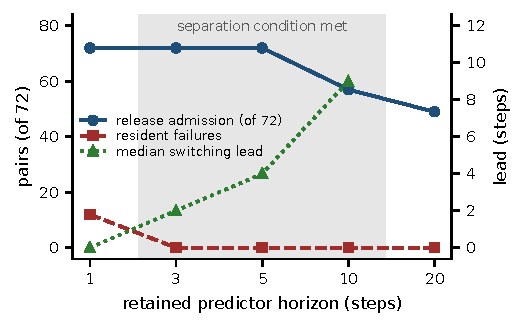
\includegraphics[width=0.99\columnwidth]{fig10_horizon_contract.pdf}
\caption{The retained check's horizon defines a usable interval rather than a
threshold.  Pooled V3 cohort, 72 snapshot--state pairs, with attack,
snapshots, and deployment states fixed; shading marks the horizons meeting the
predeclared separation condition.  At horizon 1 the retained check switches
with zero lead and still leaves 12 failures; at horizon 20 the release check
rejects so many candidates that no poisoned failure remains to separate.}
\label{fig:horizon-contract}
\end{figure}

In the independent audit, permanent raw release failed on 6/24,
3/23, and 10/24 accepted pairs.  Resident predictive authority repeats the
same five-step raw-policy prediction at every physical step and switches on
exactly those 19 paired states, four steps before failure; no physical failure
remained.  In contrast, the one-step resident kernel failed on 14 pairs despite
79 interventions and reached an empty kernel 41 times.  Repeated five-step
prediction therefore provided an effective recoverability trigger; one-time
authorization and one-step filtering did not.

\subsection{Reward-Influence Geometry and Optimizer Boundary}

We validated the reward-influence analysis on an unclipped cartpole batch
from the learner indexed by seed 2040.  Reconstructing the implemented
gradient from Equation~\eqref{eq:normalized-update} has error
$2.78\times10^{-17}$, and across 22 release-gate halfspaces the largest
discrepancy between an SOCP witness and its computed support is
$1.07\times10^{-9}$.  Audited on all 36 poisoned V3 batches, the homogenized
clipped formulation yields verified support witnesses on 22/36, where the
earlier premises admitted 0/36.  Exact batch support nevertheless did not
explain the successful multi-batch attack: the physical experiment evaluates
the fixed target and bounded attacker without establishing joint gate
optimality of the \(\tanh\) rule.  Appendix~\ref{sec:appendix-influence}
reports the full implementation audit and its parameter-clipping boundary.

\subsection{Cross-System Reward-Record Poisoning}

We next tested the lifecycle failure with updates produced by an online
learner: a Gaussian residual actor on a trusted controller, with standard
reward-to-go REINFORCE gradients computed from PyBullet transitions.  A backup
action filter protects the adaptation trajectory, and deployment then audits
the raw learned snapshot, the object requiring lifecycle admission.  Training,
certificate, calibration, and deployment states used disjoint run indices; all
mechanisms within a training realization shared paired state sets; and attack
directions and hyperparameters were fixed on a development realization before
the three-run audits.  The exact tests operate at the paired
deployment-state-block level conditional on the three learned snapshots, so
their $p$-values summarize within-snapshot discordance, and Wilson and
paired-block bootstrap intervals have the same conditional scope.

\begin{table*}[t]
\centering
\caption{Paired reward-record poisoning and snapshot admission. ``Commit''
denotes finite-horizon admission; permanent mechanisms use the common-state
audit in Fig.~\ref{fig:unified-frontier}. Raw-snapshot rewards after failure
are descriptive, not utility comparisons.}
\label{tab:end-to-end}
% Auto-generated by generate_tdsc_result_table.py; do not edit.
\begin{tabular}{llrrrr}
\toprule
System & Mechanism & Learner seeds & Rollouts & Violations & Mean reward \\
\midrule
Cartpole & Clean REINFORCE & 3 & 188 & 1 & $-0.197$ \\
Cartpole & Poisoned action-only & 3 & 188 & 38 & $-1.269$ \\
Cartpole & Poisoned commit & 3 & 188 & 0 & $-0.102$ \\
Cartpole & Always-freeze & 3 & 188 & 0 & $-0.117$ \\
\midrule
Quadrotor & Clean REINFORCE & 3 & 72 & 0 & $-0.030$ \\
Quadrotor & Poisoned action-only & 3 & 72 & 68 & $-0.170$ \\
Quadrotor & Poisoned commit & 3 & 72 & 0 & $-0.060$ \\
Quadrotor & Always-freeze & 3 & 72 & 0 & $-0.029$ \\
\bottomrule
\end{tabular}

\end{table*}

Table~\ref{tab:end-to-end} reports the paired outcomes for both systems.
On cartpole, the clean learner violates 1/188 admitted rollouts and the
poisoned action-only learner violates 38/188.  There are 37 paired poison-only
failures and no clean-only failures (two-sided exact paired
$p=1.455\times 10^{-11}$).  Both commit admission and always-freeze have zero
observed violations.

On two-dimensional quadrotor, clean learning has 0/72 violations while
reward-only poisoning causes 68/72, all delayed, across all three training
realizations (68 poison-only, zero clean-only, two-sided exact
$p=6.776\times10^{-21}$).  Every one of those failures is delayed past
adaptation, so protected execution reports nothing about any of them: the
separation follows the authority transition rather than the platform.  Commit
admission and always-freeze again have zero observed violations, and the gate
retains $0.55$, $0.40$, and $0.70$ of the poisoned pending updates, which
establishes update availability under attack rather than benign learning
utility.

\emph{Learned-baseline variant.}  Replacing REINFORCE's constant batch-mean
baseline with a learned per-state linear value baseline, under a protocol
fixed before execution and retaining the same Monte Carlo return, residual
actor, score function, and reward-record channel, poisoning caused 40/126
raw-release failures across three independent training runs, against 2/126 for
paired clean release, with commit admission and always-freeze at 0/126 (38
poison-only, zero clean-only, two-sided exact $p=7.3\times10^{-12}$).  This is
a robustness check within the Monte Carlo policy-gradient family, not a
distinct learner family: off-policy and bootstrapped learners change the
attack channel through a temporal-difference target, so the official-PPO audit
below remains the learner boundary.  These rates use the full 42-state
envelope ($126=3\times42$) without initial-acceptance filtering and are not
directly comparable to the filtered 120-pair confirmation cohort.

\emph{Non-singleton adaptation set.}  Adding the observation-FDI channel of
Section~\ref{sec:threat} to the reward-record attacker (a pole-angle bias of
radius $\rho$, so the protective kernel ranges over a box of half-width
$\rho$, about $\pm2.3^\circ$ at $\rho=0.04$) left the release certificate and
deployment states unchanged and preserved the contract separation at every
non-singleton radius.  Poisoned raw release failed on 44/126 and 61/126 pairs
at $\rho=0.02$ and $0.04$, against 4/126 and 3/126 for clean release, with
commit admission and always-freeze at 0/126; the near-singleton reference at
$\rho=0.005$ was 41/126 versus 5/126.  Failure counts were non-monotone across
training realizations, while the kernel remained nonempty throughout the grid.

\subsection{Reward-Record Integrity and Detectability Boundary}

We evaluated attack detectability separately from deployment failure.  Four
checks were fixed on the clean development run indexed by seed 2070.  The
frozen checks were then evaluated on 84 clean and 84 poisoned batches from
seven independent training runs.

\begin{table}[t]
\centering
\caption{Frozen reward-integrity audit.  Rates are batch-level true- and
false-positive rates (TPR/FPR) across seven training runs.  Each check requires
the stated defender assumption.}
\label{tab:reward-integrity}
\footnotesize
\begin{tabular}{@{}p{0.27\columnwidth}p{0.43\columnwidth}p{0.17\columnwidth}@{}}
\toprule
Check & Required trusted information & TPR/FPR\\
\midrule
Reward recomputation & Authenticated transition and deterministic reward
& 1.000/0\\
Known-sign check & Task guarantee that reward is nonpositive & 0.905/0\\
Scalar envelope & Clean development range transfers & 0.917/0.036\\
Batch-mean envelope & Clean batch mean transfers & 0.012/0.036\\
\bottomrule
\end{tabular}
\end{table}

Table~\ref{tab:reward-integrity} shows that trusted recomputation blocks every
evaluated edit, and even task-specific scalar checks detect over 90\% of
poisoned batches.  The ineffective batch-mean envelope shows why a generic
``monitor the average'' statement is not enough: detection depends on reward
semantics and trusted inputs.  Cryptographic origin binding would also reject
post-producer mutation if the trusted producer signs the reward together with
its transition, action, and time.  That producer remains within the trusted
computing base of the evaluated threat model.

Temporal and moment-preserving edits tested on the development realization
satisfied their integrity constraints and moved parameters toward the harmful
target, yet each caused 0/24 raw-release failures.  The effective fixed attack
was therefore readily detectable by the task-aware checks.  Authentication and
trusted reward recomputation provide upstream controls; commit admission and
resident predictive authority provide downstream containment.

\emph{In-loop known-sign gate.}  We placed the same known-sign check inside the
update loop and froze batches that violated the nonpositive reward guarantee.
Across three independent training runs, this gate reduced poisoned raw-release
failures from 39/126 to 0/126 and froze 35 of 36 poisoned batches.  The paired
defended-versus-undefended test gave $p=3.6\times10^{-12}$.  The gate froze no
clean batch but approached always-freeze availability under attack.  It detects
the sign-violating effective attack, while the sign-respecting variants evade
the check and independently caused no deployment harm.  This gate implements
the measured detectability boundary.

\subsection{Runtime Escape Conditions and Their Cost}

Permanent runtime filtering provides a second architectural response.  Its
certificate covers the composed policy $F\circ\pi$, allowing the filter to
contain raw-policy failure before physical execution.  We compared permanent
and snapshot contracts on a result-independent pool of 144 states from three
disjoint run indices.  For each training realization the common operating set
held states certified for both freeze and the committed snapshot at horizon
100 and guard 0.003, and eight order-spanning states were evaluated from
identical state/reset pairs, giving each mechanism 24 paired rollouts and 2400
possible steps.


\begin{figure*}[t]
\centering
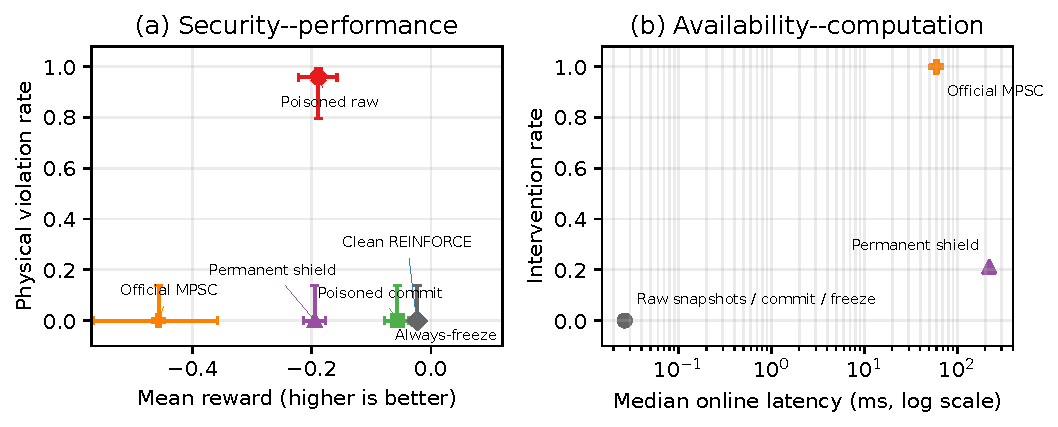
\includegraphics[width=0.94\textwidth]{tdsc_security_availability_frontier.pdf}
\caption{The unified frontier on the same paired state blocks.  Error bars in
(a) are 95\% Wilson intervals for violation rate and paired-block bootstrap
intervals for mean rollout reward, conditional on the three locked learner
snapshots.  Panel (b) separates the negligible raw
policy latency from the permanently-online protection cost; raw, commit, and
freeze mechanisms overlap near 0.026 ms and zero intervention.}
\label{fig:unified-frontier}
\end{figure*}

Table~\ref{tab:unified-frontier} in
Appendix~\ref{sec:appendix-frontier} and Fig.~\ref{fig:unified-frontier} show
the resulting separation.  The poisoned
raw snapshots violate 23/24 rollouts and complete only one.  Clean, commit,
freeze, the permanent five-step backup shield, and Safe-Control-Gym's
official linear model predictive safety certification (MPSC) mechanism all
have zero observed failures and complete 24/24.
The shield intervenes on 511/2400 steps with no rejection, while MPSC
intervenes on 2400/2400 with no infeasible solve, at median online latencies
of 222 and 60 ms against 0.026 ms for raw snapshot evaluation.  These are
single-process wall-clock measurements, not worst-case execution-time
guarantees.

The safe mechanisms differ in utility.  Mean reward ordered freeze, clean,
commit, shield, MPSC from $-0.023$ to $-0.457$; every paired rollout delta
relative to freeze had a bootstrap 95\% interval excluding zero, and no
mechanism improved on freeze in any of the 24 blocks.  These values
characterize the attack-evaluation frontier; the benign adaptation audit below
evaluates learning utility separately.



Table~\ref{tab:commit-availability} in
Appendix~\ref{sec:appendix-boundaries} makes the snapshot-admission cost
explicit: common operating-set coverage is 99.3\%, 100.0\%, and 90.3\% across
the three training runs, and trusted-state admission took 8.49--9.32\,s per
run.  Offline commit therefore avoids permanent per-action computation but
pays finite certificate coverage and update latency.  The comparison distinguishes three
contracts: certify a snapshot before raw deployment, retain a filter
permanently, or stop adapting.

\subsection{Sizing a Release Gate}

The measurements above support a contract-specific rule.  Two decisions are
made at the authority transition, and each has a measurable input.

\emph{Retiring authority.}  The release evidence must re-establish every
premise the transition changes (Proposition~\ref{prop:transfer}).  Here those
premises are authority and horizon: the accepted check bounds the raw policy
for five steps, and only while it can still hand control back.  Re-running the
same check discharges neither obligation, which is why permanent raw release
failed on states it had accepted, with and without an attacker.

\emph{Retaining authority.}  The lookahead then has a lower and an upper edge,
and both are measurable on the deploying system without knowing the attack.
The lower edge is the lead time the trusted baseline needs to recover: at
horizon 1 the retained check switched with zero lead and still left 12
failures, whereas horizons 3 to 10 switched 2 to 9 steps early and left none.
The upper edge is the admission the operator can afford to lose: raising the
horizon from 5 to 10 and to 20 rejected 15 and 23 of the 72 candidates the
shorter checks admitted.  Both edges come from the sweep of
Fig.~\ref{fig:horizon-contract} applied to the deployer's own baseline and
candidate pool, so the gate can be sized from the recovery dynamics of the
backup rather than from an attack model.

\subsection{Boundaries and Validity}

Four locked audits bound the result.  A trusted state anchor shrinks
certificate uncertainty without sanitizing the reward record: every anchor
period retains all 16 certificate centers, has 0/24 violations on new paired
blocks, and improves no reward over freeze.  Against the official pretrained
PPO policy, which is safe on 72/72 held-out rollouts, the locked
$L_\infty\le0.5$ budget produced 1/24 poisoned failures at one checkpoint and
0/24 at another, so the audit showed checkpoint-level update redirection
without a stable deep-PPO unsafe-policy effect.  Under a benign $0.003$\,N
differential actuator bias, freeze, clean adaptation, and the
certificate-gated learner were all violation-free; the gate accepted a nonzero
update in 11/12 batches but improves no paired rollout over freeze, so
certificate acceptance did not establish useful adaptation.  A fourth audit bounds how far the finite certificate transfers.  On 1728
snapshot--state pairs at the pre-existing 100-step, 0.003-guard configuration,
CasADi certified 1293, none of which violated the PyBullet state box within
100 steps, while the poisoned raw snapshots violated 403/432 pairs at
certificate coverage 0.062 --- informative rejection rather than vacuous
evidence.  The guard margin is what separates the two regimes:
without it the poisoned snapshots produced 1, 2, and 1 false acceptances at
horizons 20, 50, and 100, and every locked positive guard removed the observed
false acceptances while rejecting more physically safe pairs
(Appendix~\ref{sec:appendix-coverage}).  The gate therefore has a second
measurable knob beyond horizon, calibrated against model mismatch rather than
against an attacker.

The CasADi gates use fixed finite state
sets while physical outcomes use independent PyBullet rollouts; they are
sampled finite-horizon certificates, not continuous-state invariant-set
proofs.  Realized state violations and pre-clip saturation are reported
separately.  Appendix~\ref{sec:appendix-boundaries} gives the full figures.

\section{Third-Party Shield-Retirement Case Study}
\label{sec:third-party}

The controlled contract in Section~\ref{sec:study} isolates the mechanism.
This section examines the same integrity boundary in an independently
published lifecycle that retires runtime authority.
Carr et al.~\cite{carr_partial_shielding_2023} (AAAI 2023) train a
policy-gradient agent behind a Storm belief-support shield in a partially
observable gridworld.  Their lifecycle later removes the shield either
suddenly or smoothly and compares the released policy with retained-shield
and no-shield controls.  We use the official public implementation and modify
only learner-visible reward records.  The attacker writes
$r'=r+\xi$, with $|\xi|\le\delta$ per record, before the trusted update.
States, observations, shield semantics, dynamics, learner code,
hyperparameters, and evaluation follow the upstream implementation.  The
artifact itemizes every instrumentation and attack patch.  REINFORCE training
runs for 5000 episodes, with retirement at episode 1000.  The TF-Agents
proximal policy optimization (PPO) pipeline retires the shield after $10^5$
environment steps.

\paragraph{Lifecycle fidelity.}
On the obstacle domain ($N{=}6$), the clean condition reproduces the
qualitative ordering of Carr et al.'s Table~1 for REINFORCE: shield retained
0/0 violations during/after training, smooth 326/675, sudden 3277/3784, and
no-shield 3798/3784.  Shield $<$ smooth $\ll$ sudden $\le$ no-shield is the
ordering reported by Carr et al., establishing the lifecycle fidelity of the
instrumented implementation.

\paragraph{Causal isolation at the retirement boundary.}
Under a locked protocol (artifact amendment v1.3), poisoning is confined to
the shielded bootstrap phase.  Reward-record mutation is active only while
the shield enforces the action mask and stops at retirement.  All subsequent
learning is clean.  We evaluate the raw policy at
the switch instant before any unshielded learning (1000 episodes) and again
after the full training budget (5000 episodes).  Each independently trained
clean/poisoned pair is one training-level replicate; configured seeds serve
only as run indices.  Table~\ref{tab:carr-isolation} and
Fig.~\ref{fig:carr-isolation} report the provenance-complete pairs.  A pair is
\emph{positive} when the poisoned at-retirement rate exceeds its clean pair by
at least $0.15$ and the paired McNemar exact test gives $p<0.01$.  All other
outcomes are \emph{non-positive}; \emph{protective} denotes a lower poisoned
rate.

\begin{table}[t]
\centering
\caption{Retirement-boundary causal isolation on the third-party lifecycle
(obstacle, REINFORCE, sudden).  Each row is a provenance-complete paired
training run.  Poisoning stops at retirement, and all later training is
clean.  At-retirement evaluates the raw policy at episode 1000; final
evaluates it at episode 5000.  Rates are violation fractions.}
\label{tab:carr-isolation}
\small
\begin{tabular}{@{}ccccc@{}}
\toprule
 & \multicolumn{2}{c}{at retirement} & \multicolumn{2}{c}{final}\\
\cmidrule(lr){2-3}\cmidrule(lr){4-5}
configured seed & clean & poisoned & clean & poisoned\\
\midrule
1 & 0.216 & 0.777 & 0.236 & 0.235\\
2 & 0.484 & 0.763 & 0.234 & 0.751\\
3$^a$ & 0.241 & 0.242 & 0.747 & 0.228\\
\bottomrule
\end{tabular}
\vspace{1pt}\par\footnotesize $^a$An earlier run-index-3 clean summary
duplicated a separate fix-check record and is excluded.  This row reports a
fresh clean/poisoned pair generated under the locked configuration.  The
archived poisoned realization (0.748 at retirement) lacks a provenance-valid
clean endpoint and is excluded from paired inference.
\end{table}

Two of the three provenance-complete pairs had higher raw-policy violation
rates at retirement under poisoning, by factors of $3.6$ and $1.6$.  The fresh
third pair was unchanged ($0.241\rightarrow0.242$).  Physical violations
remained zero throughout protected execution.  The positive outcomes located
latent policy damage before unshielded learning.  The fresh pair showed that
the fixed attack can fail in a low-disagreement retirement state.  After 4000
episodes of clean post-retirement learning, one positive pair recovered
($0.235$ vs.\ clean $0.236$), one remained worse
($0.751$ vs.\ $0.234$), and the fresh non-positive pair reversed
($0.228$ vs.\ $0.747$).  We denote clean raw-policy/shield disagreement at
retirement by $D_{\mathrm{ret}}$.  In the two positive pairs,
$D_{\mathrm{ret}}$ was $0.025$ and $0.047$ and rose to $0.113$ and $0.109$
under poisoning.  The fresh non-positive pair also had low clean disagreement
($D_{\mathrm{ret}}=0.013$), separating available headroom from attack success.

\begin{figure*}[t]
\centering

\includegraphics[width=\textwidth]{fig6_retirement_isolation_summary.pdf}
\caption{Causal isolation on the third-party lifecycle (REINFORCE, obstacle,
sudden, provenance-complete paired runs).  (a) At-retirement violation fraction of the raw
policy; (b) at-retirement raw-policy/shield disagreement; (c) final
violation fraction after clean post-retirement learning.  Poisoning is
confined to the shielded bootstrap phase.  The run-index-3 bars show the fresh
pair in Table~\ref{tab:carr-isolation}.}
\label{fig:carr-isolation}
\end{figure*}

\paragraph{Learner boundary.}
The same contrast attack ($\delta{=}2$) was evaluated on the third-party PPO
pipeline with action masking and sudden retirement.  It raised post-removal
violations in one of three paired runs, from 1178 to 2439
(McNemar exact $p=2.6\times10^{-149}$).  The first-violation episode changed
from 6 to 0.  The other two runs were unchanged ($p=1.00$ and $0.96$).  In a
separate ten-run shield-on-only isolation
battery, the run indexed by configured seed 101 was positive
($0.219\rightarrow0.754$ at retirement; McNemar exact
$p=3.7\times10^{-113}$), while the other nine entered a high-violation ceiling
regime (clean $0.728$--$0.760$) and were either protective or unchanged.
Figure~\ref{fig:ppo-isolation} reports the full battery.  A ten-run full-phase
PPO battery likewise placed every clean policy near the retirement ceiling
($0.73$--$0.77$) and yielded no positive outcome on the primary retirement
metric.  Its final metric captured a different effect: all ten poisoned
policies remained unsafe ($0.49$--$0.77$), whereas nine clean policies recovered
to approximately $0.22$ under continued learning.

A ten-run shield-on-only battery on off-policy soft actor-critic (SAC)
provided a complementary boundary.  Three runs were positive
($0.207\rightarrow0.561$, $0.218\rightarrow0.513$, and
$0.479\rightarrow0.954$; paired McNemar exact $p<10^{-40}$ for each), three
were protective, and four were unchanged.  All ten clean SAC policies had low
retirement disagreement rather than occupying the ceiling regime.  Four
extension runs generated on a second host were non-positive.  The fixed
attack therefore affected individual PPO and SAC training realizations without
producing reliable success within either family.

\begin{figure*}[t]
\centering

\includegraphics[width=0.85\textwidth]{fig6_ppo_isolation.pdf}
\caption{PPO retirement-boundary isolation on the third-party lifecycle
(shield-on-only contrast poisoning, $\delta{=}2$, paired runs indexed by
run indices 101--110,
sudden retirement).  At-retirement violation fraction of the raw policy for
clean and poisoned runs.  The run indexed by 101 is positive
($0.219\rightarrow0.754$; McNemar exact $p=3.7\times10^{-113}$); the other
nine runs land in the unsafe ceiling regime (clean at-retirement
$0.728$--$0.760$) with no paired headroom, six protective by the paired test and
three unchanged.  The dashed line marks the locked decision boundary
(poisoned at least $0.15$ above clean with paired McNemar $p<0.01$).}
\label{fig:ppo-isolation}
\end{figure*}

\paragraph{Attack budget and state dependence.}
On the full-phase REINFORCE protocol, the effect varied with attack shape,
budget, and training realization.  In the realization indexed by configured
seed~2, $\delta{=}2$ raised post-removal violations from 1127 to 3762
($3.3\times$; McNemar exact $p$ below numerical reporting precision).
Increasing the budget to $\delta{=}10$ produced 3766 violations.  In the
realization indexed by seed~3, $\delta{=}2$ was unchanged (2482 vs.\ 2471;
$p=0.84$), whereas $\delta{=}10$ raised violations to 3700
($p=8.4\times10^{-138}$).  The realization indexed by seed~1 began near the
unsafe ceiling (75.7\%) and showed no added damage at either budget.  Shape
controls were also state-dependent.  The bias variant was protective in the
ceiling realization.  The risk variant was protective in two realizations and
raised violations from 1127 to 2457 in the realization indexed by seed~2.

An independent Linux-host batch with identical dependency versions contained
one low-clean-violation realization and two ceiling realizations.  The former
showed the contrast effect at retirement ($0.232\rightarrow0.501$) and after
removal (1157 $\rightarrow$ 2451; $p=4.6\times10^{-159}$).  The latter two were
unchanged at $\delta{=}2$ and protective at $\delta{=}10$.  The run index of
the low-clean-violation regime differed across hosts.  Repeating the clean
configuration also entered a different trajectory mode ($0.776$ rather than
$0.232$ at retirement).  Dose comparisons are therefore confined to the
locked local batch.  The independent batch shows that attackability follows
the realized retirement state more closely than the nominal seed identifier.

\begin{figure*}[t]
\centering
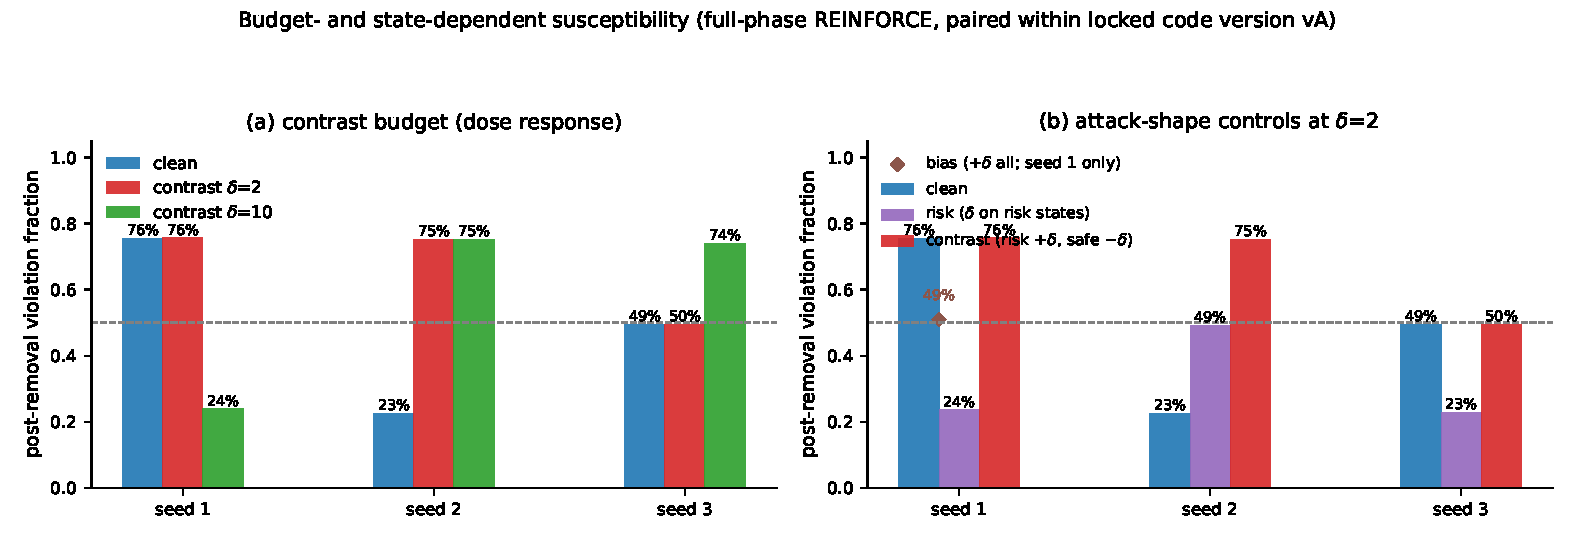
\includegraphics[width=\textwidth]{fig7_dose_response.pdf}
\caption{Budget- and state-dependent effects on the full-phase REINFORCE
protocol (paired within one locked code version).  (a) Contrast
attack dose response; (b) attack-shape negative controls at $\delta{=}2$.
The run-index-2 realization saturates at $\delta{=}2$; the run-index-3
realization requires $\delta{=}10$; the ceiling realization shows no additional damage at
either budget, and bias/risk controls are protective or strictly weaker.}
\label{fig:dose-response}
\end{figure*}

\paragraph{Escape condition.}
Under the same full-scope poisoning used in the full-phase battery, a retained
shield kept physical violations at zero before and after training in all three
paired runs.  The corresponding sudden-retirement runs exposed final violation
fractions of $0.490$, $0.752$, and $0.744$ after removal.  Resident authority
therefore contained the downstream
consequence of full-scope contamination; removing it exposes the same
consequence as an unsafe released policy.

\paragraph{Interpretation.}
Carr et al.'s workflow supplies the lifecycle component: protected bootstrap
followed by retirement of the shield's action authority.  The controlled
study in Section~\ref{sec:study} supplies the adversarial-provenance
mechanism.  Their composition exposes an integrity boundary at authority
transition.  Carr et al.'s original evaluation concerns shield-removal
behavior under unpoisoned learning; the case study concerns evidence reuse
across the same transition under adversarial update provenance.
Absolute rates differ across instrumented and non-instrumented code versions
because the unmasked-disagreement probe requires an independent belief
tracker; all clean-vs-poisoned comparisons above are paired within a locked
code version and are unaffected by that version change.

Training outcomes also varied across platforms.  In a ten-run REINFORCE
shield-on-only battery on Linux, three low-clean-violation realizations were
positive ($0.240\rightarrow0.533$, $0.234\rightarrow0.744$, and
$0.229\rightarrow0.763$), while seven ceiling realizations showed no added
damage.  By contrast, the fresh pair in Table~\ref{tab:carr-isolation} was
non-positive despite low clean disagreement.  The same configured seed and
code can enter different trajectory modes across hosts or backends.  We
therefore treat each independently trained clean/poisoned pair as a replicate
and use nominal seeds only as run indices.  Episode-level McNemar tests
describe outcomes conditional on a trained pair; the multi-run batteries
provide the training-level replication evidence.

The broader cross-tabulation reinforced this state dependence.  Across 53
locked paired runs spanning both scopes, all three learner families, and both
domains, 12 of 20 runs with clean at-retirement violation below $0.5$ were
positive, whereas none of 33 ceiling runs was positive
(Fig.~\ref{fig:two-by-two}).  The eight low-rate exceptions comprise six SAC
runs and two protective runs in the second environment.  Low clean violation
therefore marks available headroom but does not determine the attack outcome.

The 50 obstacle runs with disagreement instrumentation provided a sharper
retirement-state marker.  Clean $D_{\mathrm{ret}}$ was strongly associated
with clean violation (Spearman $0.976$,
$p=1.3\times10^{-33}$) and negatively associated with attack headroom
(Spearman $-0.547$, $p=3.9\times10^{-5}$).  Every positive outcome had clean
$D_{\mathrm{ret}}\le0.047$, while non-positive outcomes extended to $0.111$.
Under the fixed bands, all 11 positive outcomes fell in the low-disagreement
region ($D_{\mathrm{ret}}<0.06$), and none of 32 high-disagreement runs was
positive.  The area under the receiver operating characteristic curve (AUC)
was $0.953$
(Mann--Whitney $p=5.5\times10^{-6}$).  Family-stratified counts clarify this
statistic.  REINFORCE had seven positive low-band runs and 13 non-positive
high-band runs.  PPO had one positive low-band run and 19 non-positive
high-band runs.  All ten SAC runs were low-band, with three positive and seven
non-positive outcomes.  Thus high disagreement acted as a
strong exclusion condition in this corpus, whereas low disagreement defined
an opportunity region.  Eleven of 18 low-band corpus runs were positive; the
fresh pair, analyzed separately from the 50 disjoint namespaces, gave an
additional low-band non-positive realization.

The protocol chronology bounds the statistical interpretation.  The
$0.06/0.09$ bands were fixed after analysis of 46 existing obstacle rows and
before four SAC extension pairs with run indices 407--410.  All four
extensions were low-band and non-positive.  They strengthened the
non-sufficiency result without prospectively testing high-disagreement
exclusion.  Accordingly, AUC $0.953$ describes discrimination within the
combined locked corpus, not external classifier validation.  Because
$D_{\mathrm{ret}}$ is measured after the shielded bootstrap, it characterizes
the realized retirement state.  An online attack trigger would require
earlier disagreement trajectories that predict the eventual opportunity
region.  The marker is also obstacle-scoped.  Two protective runs in the
second environment had clean disagreement $0.476$ and $0.157$ despite clean
violation below $0.5$.

\begin{figure*}[t]
\centering
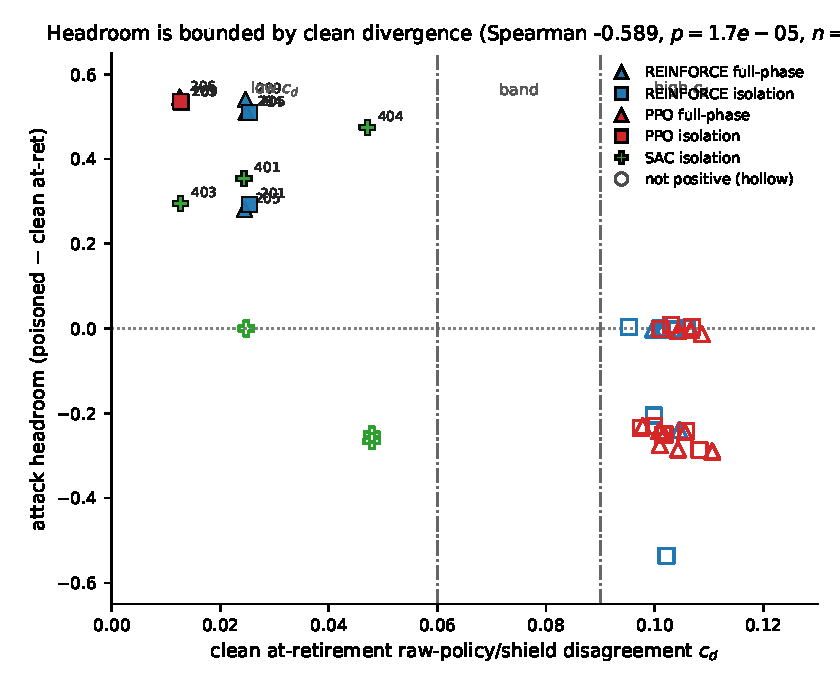
\includegraphics[width=0.72\textwidth]{fig9_mechanism_divergence.pdf}
\caption{Clean at-retirement raw-policy/shield disagreement marks an
opportunity region across the obstacle corpus (both scopes, all three learner
families).  Each point is one paired clean/poisoned run; filled markers meet
the positive-outcome rule, and hollow markers do not.
Filled markers all have clean disagreement $\le0.047$; the dashed lines mark
the fixed low/high disagreement bands ($<0.06$ and $\ge0.09$).  No
high-disagreement run is positive, while seven of 18 low-disagreement runs are
non-positive.}
\label{fig:mechanism}
\end{figure*}



\begin{figure*}[t]
\centering

\includegraphics[width=\textwidth]{fig8_2x2_susceptibility.pdf}
\caption{Two-by-two opportunity-region cross-tabulation across all locked
paired runs (both scopes, all three learner families, both domains).  Each
point is one paired clean/poisoned run; filled markers meet the positive rule
(poisoned at-retirement at least $0.15$ above clean at retirement with paired
McNemar exact $p<0.01$), hollow markers do not.  The dashed rule line is
$y=x+0.15$ and the vertical dashed line marks the clean at-retirement $0.5$
boundary: positive outcomes concentrate below $0.5$, and no ceiling run is
positive.}
\label{fig:two-by-two}
\end{figure*}

\paragraph{Environment boundary.}
On a second gridworld of the same third-party suite (surveillance, $N{=}6$,
$R{=}3$), a clean reproduction again satisfied the authors' lifecycle
ordering: shield retained
$0/0$, smooth $0.129$, sudden $0.246$, and no-shield $0.252$ (retained $<$
smooth $\ll$ sudden $\le$ no-shield).  The fixed contrast attack at
$\delta{=}2$ raised post-removal violations in one of three independent paired
runs ($0.000 \rightarrow 0.272$, McNemar exact $p=2.6\times10^{-82}$) and was
protective in the other two ($0.267 \rightarrow 0.000$,
$p=8.4\times10^{-81}$; $0.135 \rightarrow 0.038$,
$p=1.3\times10^{-15}$).  The lifecycle ordering extended to the second
environment, whereas the exploit effect remained environment- and
realization-dependent.

\section{Related Work}
\label{sec:related}

\emph{Assurance cases and change impact.}
System change does not invalidate every assurance artifact.  It requires
change-impact analysis to identify which claims depend on premises that no
longer hold.  Kelly and McDermid give an impact analysis for deciding which
parts of an argument a change invalidates~\cite{kelly_safety_case_maintenance_2001}, and
dynamic safety cases carry it into operation so assurance is re-argued through
life~\cite{denney_dynamic_safety_cases_2015}.  That literature asks whether
engineers correctly re-argue safety after a known change.  We instantiate that
maintenance problem at two controller handoffs: extrapolating a bounded
raw-policy release test and transferring control to a fallback are separate
change-impact events with distinct premises.

\emph{Runtime assurance and safe controller updates.}
Safety filters and shields form a design space, and we position against it as
a whole~\cite{brunke_safe_learning_survey_2022}.
Simplex architectures retain a decision module and a baseline trusted under
the system fault model during online upgrades~\cite{seto_simplex_1998}; neural
and barrier-based Simplex add online retraining, reverse switching, and
switching conditions under bounded model error
\cite{phan_neural_simplex_2020,damare_bb_simplex_2025}; and MPSC and runtime
shields preserve recoverability or prevent unsafe actions
\cite{wabersich_linear_mpsc_2018,didier_adaptive_mpsc_2021,
alshiekh_shielding_2018}.  These lines already establish that safe switching
requires a recoverability or invariant-set argument.  Our controlled audit
deliberately evaluates a weaker mechanism---repeated lookahead for the outgoing
raw policy without a recovery certificate for the receiver---to measure the
consequence of treating those claims as interchangeable.  Policy repair, safe projection, joint
controller/certificate repair, robust conformal transfer, and shielded
sim-to-real transfer instead establish evidence for the deployment object
before use \cite{zhou_runtime_policy_repair_2020,lu_repair_preservation_2024,
chow_safe_policy_2021,yu_certificate_repair_2025,
mirzaeedodangeh_safe_updates_2026,hsu_sim_lab_real_2023}.

\emph{Shield retirement and attacked states.}
Könighofer et al.~\cite{konighofer_online_shielding_2022} establish the
non-adversarial half of this observation: policies trained under an online
shield inflict more unshielded violations than conventionally trained ones, so
shielding must be applied during execution.  They further note that a
finite-horizon shield needs sufficient lookahead, or the agent reaches states
in which every action is unsafe; the 41 empty kernels under our one-step action
filter instantiate that situation.  Our horizon sweep quantifies the tradeoff
between warning time and admission.  The duration study then shows why
raw-policy warning cannot replace the recoverability condition already required
by runtime-assurance designs: 19 paired failures occurred only under raw
execution, whereas seven occurred only after the lookahead switcher transferred
control to the LQR fallback.  Because the experiment evaluates no recovery
certificate, these outcomes do not locate the handoff states relative to a
recoverable set.  Carr et al.~\cite{carr_partial_shielding_2023} study a partially observable
bootstrap-to-retirement lifecycle and compare sudden with smooth shield
removal under trusted learning signals.  We reuse that published lifecycle as
a third-party case study and add bounded reward-record poisoning during the
protected bootstrap.  Carr et al. do not claim that a five-step test certifies
permanent execution; their workflow establishes the retirement setting, while
our paired experiment evaluates whether bootstrap-only data corruption can
alter the policy exposed at retirement.

Secure estimation characterizes when sensor attacks can be detected or
corrected~\cite{pasqualetti_attack_2013,fawzi_secure_2014}, and severe-attack
CBF filtering constructs plausible-state sets and safe-action kernels when the
state is not uniquely reconstructable~\cite{tan_safety_2024}; our model
consumes such a set and asks whether an adversarially updated action map stays
inside its certified kernel.  Related lines learn barriers or solve
adversarial reach--avoid problems under trusted learning signals
\cite{brunke_barrier_learning_2022,
capone_bandit_safe_control_2025,wu_certifying_2022,pham_certified_2024,
hsu_isaacs_2023,nguyen_gameplay_2024}.  Table~\ref{tab:delta} in
Appendix~\ref{sec:appendix-delta} places the closest work on the three axes
this paper combines.

\emph{Policy and reward poisoning.}
Policy poisoning has been studied in batch reinforcement learning and
control~\cite{ma_policy_poisoning_2019}; online attacks perturb rewards under
an $\ell_\infty$ budget and adapt to the
learner~\cite{zhang_reward_poisoning_2020}; extensions cover policy-gradient
and black-box deep learners, and targeted poisoning can teach a chosen policy
\cite{sun_online_rl_poisoning_2021,xu_deep_reward_poisoning_2025,
rakhsha_policy_teaching_2020,everitt_corrupted_reward_2017}.  None of this
line places the learner behind a runtime shield.

\emph{Backdoors on shielded and classical controllers.}
Jiang et al.\ implant backdoors in formal-language-guided \emph{safe} RL
policies, so that a trigger state reached at runtime produces a safety
violation~\cite{jiang_backdoor_safe_rl_cps_2024}.  This is the closest prior
composition, and the difference matters: their trigger must survive a shield
that is never retired, whereas our attack plants no input-triggered behavior.
Its effect becomes observable when protection is absent---after a bounded
release test in the controlled audit, or after shield retirement in the
third-party workflow.  The manipulated object is the learning record rather
than a deployment input.
BADControl poisons operational data in proportional-integral-derivative (PID)
and LQR loops to implant a vulnerability activated by a physical
trigger~\cite{burbano_badcontrol_2026}, which shares the trigger structure
without the learner or the shield.  Where online
reward-poisoning defenses model adaptive attacker--defender interaction
\cite{nika_reward_defense_2023}, we separate provenance, trusted
recomputation, detection, commit admission, and runtime containment.

Appendix~\ref{sec:appendix-support} applies classical homogenization and
second-order-cone feasibility \cite{schaible_fractional_duality_1976,
agrawal_dqcp_2020,bauschke_homogenization_2023,belloni_soc_feasibility_2008}
to the normalized image of a centered reward-to-go zonotope.

\section{Discussion and Limitations}

The clean cohort isolates horizon extrapolation: its five-step test directly
evaluates the final raw-policy snapshot without shield intervention, but does
not support a 120-step claim.  The duration study isolates a different premise:
warning about the outgoing policy does not establish LQR recovery from the
transfer state.  Reward-record poisoning stresses both contracts but creates
neither obligation.

In the Carr corpus, positive outcomes occurred only at low retirement-state
disagreement, but that region also contained non-positive outcomes.  The
53-run accounting (12 positive, 20 protective, and 21 unchanged) therefore
supports a conditional, not uniform, effect.  Trusted recomputation, commit
admission, and recovery-aware switching address different premises and incur
different coverage, latency, and intervention costs.

Adaptation should justify those costs by paired task benefit over freeze.  The
locked benign audit stopped after 0/12 improvements, so the evaluated settings
provide no such utility basis; this result does not extend to unevaluated
deployments.

\subsection{Limitations}
\label{sec:limits}

\emph{The marker is descriptive, not an attacker trigger.}  Retirement-state
disagreement is observed only after bootstrap.  Two historical REINFORCE
membership decisions also lack an executable deduplication rule, so we omit
the affected corpus statistic and counts.  The reproducible high-band result
is an obstacle-scoped exclusion condition, not a validated predictor; holding
out SAC identifies only 3 of 10 outcomes.

\emph{The formal results have bounded verification scope.}
The evidence record in Section~\ref{sec:threat} is dependency bookkeeping, not
a proof calculus, and yields no empirical result.  The linear parameter gate is
exact only on its finite abstraction; its continuous lift requires a justified
reachable-set cover, regularity and model-error bounds, and a robust margin.
The coverage audit does not establish continuous-state invariance.  Exact
reward influence covers one fixed standardized-advantage batch with global
gradient clipping, not coordinatewise clipping or multi-batch construction.

\emph{Empirical generality is bounded to Monte Carlo policy gradients.}  The
learned-baseline variant shares their return and attack channel, so it is not
an independent family.  The official Safe-Control-Gym PPO audit showed
checkpoint-level redirection without stable physical failure, and on the
third-party lifecycle PPO and SAC contained individual positive realizations
without reliable success across paired runs.

\emph{The horizon and workload claims remain experimental.}  The five-step
horizon was development-fixed, and its sweep uses the poisoned V3 cohort, not
the 20-run clean cohort.  We therefore do not estimate clean run-level failure
prevalence by horizon.  Both platforms expose recomputable deterministic
rewards; delayed labels and external KPIs motivate, but do not empirically
validate, the non-reconstructable-reward setting.

\emph{We assume access, and do not estimate its prevalence.}  The attack reads
learner state in addition to writing one scalar field
(Table~\ref{tab:trust-boundary}).  Predicate-aware edits evade the task-aware
checks; trusted recomputation closes the channel but falls outside the stated
applicability condition.  At 48 batches, switcher failures occur in two of five
controllers.  We neither certify an LQR recovery set nor identify safe handoff
states, limiting claims about prevalence and alternate switching times.

\section{Conclusion}
\label{sec:conclusion}

Conditional on bounded write access at an otherwise isolated reward-ingestion
interface, protected adaptation and raw release are different security
contracts.  After a development block locks the target, attacker, and
detector, five untouched seeds yield 27/120 poisoned permanent-release
failures versus 2/120 paired clean.  Resident predictive authority switches
before every corresponding poisoned failure and incurs 0/120 failures;
horizons 3, 5, and 10 all separate the contracts.  An independent audit finds
that a one-step resident kernel still fails on 14/71.  The result therefore
depends on recoverability, not residence alone.

The normalized reward-influence analysis characterizes the batch-local update
authority available through reward corruption.  Conic homogenization makes
positive support exact across normalization singularities and global
gradient-norm clipping, while coordinatewise parameter clipping and
multi-batch attack construction remain outside the theorem.  The broader
cartpole and quadrotor experiments,
finite-horizon commit gate, freeze, backup shield, and official MPSC then
expose the coverage, intervention, reward, and latency costs of different
escape contracts.

The integrity boundary is also part of the result.  Trusted recomputation
blocks every evaluated edit, and simple task-aware checks detect over 90\% of
poisoned batches.  Provenance or recomputation removes the upstream attack
precondition; commit admission and resident authority instead contain its
downstream consequence.  We do not claim a logging-service exploit or a
stealthy attack.

The remaining negative boundaries are part of the result.  The target was
development-fixed, the bounded \(\tanh\) perturbation is not a joint gate
optimizer, and even the extended exact-support diagnostic produces no raw
release failure.  The physical attack is established for low-dimensional Monte-Carlo
policy-gradient learners (REINFORCE and a learned-baseline variant), does not
stably transfer to official PPO, and admitted updates do not beat freeze in
the benign-adaptation smoke.
Thus resident predictive evidence is contract-bound; raw release needs
independent future coverage.


% Acknowledgments are omitted from the anonymous submission.

% Ethical Considerations and Open Science are USENIX appendices and are
% excluded from the 13-page body limit.
\clearpage
\section*{Ethical Considerations}

This paper studies an attack on safety-critical learning-enabled control.  All
experiments run in simulation using Safe-Control-Gym with PyBullet dynamics
and a public third-party gridworld implementation.  No physical plant,
vehicle, deployed industrial system, human subject, or personal data was
involved.  Reported failures are simulated constraint violations used to
compare deployment contracts.

The evaluated threat begins \emph{after} compromise of a reward-ingestion
principal in the asynchronous learning-data plane and grants only bounded
scalar writes to reward records.  Initial access, product-specific
exploitation, and evasion of log-integrity controls fall outside the artifact
and evaluation.  The experiments characterize the consequence of a
least-privilege data-integrity gap for evidence inheritance at raw-policy
release.  We therefore describe a composition weakness in an assurance
workflow rather than an exploit against an identified fielded product, and we
publish no capability that lowers the cost of obtaining the assumed access.

Stakeholders are operators of runtime-assured learning controllers, vendors of
shielding and safety-filter tooling, and the public exposed to the controlled
plant.  The main foreseeable harm from publication is that an attacker who
already holds reward-ingestion access learns that a retired shield leaves
latent policy damage exposed.  We judge the disclosure benefit to dominate:
the exposure follows from documented assurance architectures, the attack is
detected by the simple task-aware reward checks we measure, and the paper
states deployable countermeasures at both ends of the authority transition.
Origin-bound reward records and trusted recomputation remove the upstream
precondition; resident predictive authority, commit admission, and permanent
filtering contain the downstream physical consequence.

The third-party lifecycle we instrument is a published research artifact
released under an open license by its authors, used unmodified except for
documented instrumentation and reward-record patches that the artifact
itemizes.  No vendor product, hosted service, or operational deployment was
tested, so no coordinated vulnerability disclosure was owed to a third party.
We follow the USENIX Security ethics guidelines and the principles of the
Menlo Report in reporting the above.

\section*{Open Science}

We support the USENIX Security open science policy and will make every
artifact required to reproduce the reported results openly available.  The
artifact contains: (i) the experiment drivers for the controlled
Safe-Control-Gym study and the third-party shield-retirement case study;
(ii) row-level result files backing every table and figure, with source-linked
provenance columns; (iii) exact commands, run namespaces, upstream revisions,
model files, and dependency versions; (iv) locked protocol documents recording
the analysis chronology; and (v) SHA-256 checksums for all locked files.
Automated checks in the artifact audit table provenance, claim locks, and
manuscript format.

For anonymous review, the artifact is submitted as an anonymized archive
through the submission system, so the review committees can access every
component without contacting the authors.  Upon acceptance we will publish the
same artifact in a public repository with a permanent DOI under an open
license, together with the third-party upstream revision pins required to
rebuild the case-study environment.  The artifact retains the scope boundaries
stated in the paper: the trusted-anchor, certificate-coverage, timing, PPO,
benign-utility, and protocol-chronology limitations are recorded with the data
rather than removed.


\bibliographystyle{IEEEtran}
\bibliography{reference}

% Technical appendices follow the references and are excluded from the
% 13-page body limit for the initial submission.
\appendix
\section{Deferred Proofs}
\label{sec:appendix-proofs}

This appendix collects the proofs deferred from Sections~\ref{sec:model}
and~\ref{sec:gate}, in the order the results are stated, and adds the
action-filtering separation those sections refer to.

\begin{proof}[Proof of Proposition~\ref{prop:transfer}]
Each component records a premise under which the acceptance evidence was
derived.  If an authority transition removes or weakens that premise, the
original derivation does not establish the corresponding obligation under
$C_{\mathrm{deploy}}$.  Re-establishing every changed obligation supplies the
missing premises; without them, $E$ alone is insufficient.  In the evaluated
permanent-release transition, resident authority is removed and a finite check
authorizes a longer unmonitored execution, so both authority and horizon
change.  Under attack, update provenance changes as well.  Evidence carried
over from protected adaptation also changes subject, from the assured
composition to the raw policy.  The same argument applies independently to a
later handoff from that policy to a baseline controller.
\end{proof}

\begin{proof}[Proof of Lemma~\ref{lem:current-gate}]
The certified action must satisfy the certificate for every state compatible
with the attacked history.  These states form $X_{\mathcal A}(h)$, and their
common certified actions form $K_\Gamma(h)$.  Continued certified operation
therefore requires $\pi_{\theta_{t+1}}(h)\in K_\Gamma(h)$.  An empty kernel
requires rejection, freeze, rollback, or trusted information that changes the
plausible-state set.
\end{proof}

\begin{proposition}[Action filtering is not update certification]
\label{prop:action-filter-insufficient}
Let $F(v,h)$ be an action filter that returns an applied input in
$K_\Gamma(h)$ whenever the kernel is nonempty.  Consider a mechanism that
first computes $\theta^+=U(\theta_t,h)$ and then applies
\begin{equation}
    u_t=F(\pi_{\theta^+}(h),h),
\end{equation}
The mechanism accepts the update without constraining the raw updated policy
$\pi_{\theta^+}$.  If $\pi_{\theta^+}(h)\notin K_\Gamma(h)$, the applied input
can be certified while the updated learner remains uncertified.  Action-only
filtering therefore does not imply Lemma~\ref{lem:current-gate}.
\end{proposition}

\begin{proof}[Proof of Proposition~\ref{prop:action-filter-insufficient}]
The filter property gives $u_t\in K_\Gamma(h)$, so the current actuator input
can satisfy the certificate.  Lemma~\ref{lem:current-gate} instead constrains
the updated controller through
$\pi_{\theta^+}(h)\in K_\Gamma(h)$.  When this membership fails, the
certificate covers only the filtered actuator channel.  Accepting the update
under that certificate creates a stale certified policy.
\end{proof}

\begin{proof}[Proof of Theorem~\ref{thm:gate}]
Applying Lemma~\ref{lem:current-gate} pointwise to every
$h'\in\mathcal H_{\mathcal A}(h,\theta^+)$, which the soundness definition of
Section~\ref{sec:model} quantifies over, gives
$\pi_{\theta^+}(h')\in K_\Gamma(h')$ for each such history.  This is the
definition of $\theta^+\in\Theta_\Gamma(h)$.  A failed membership leaves the
updated action map uncertified at that history.  An empty kernel additionally
requires a changed information set or rejection of certified operation.
\end{proof}

\begin{proof}[Proof of Proposition~\ref{prop:parameter-gate}]
For fixed $z$, membership $\pi_\theta(z)\in[\ell_z,u_z]$ is equivalent to the
two inequalities of~\eqref{eq:parameter-gate-halfspaces}.  Enforcing them for every $z\in\mathcal Z$ implements
the lifecycle gate on the abstraction.  Parameter box constraints preserve
convexity.  A feasible or projected candidate satisfies every certified
interval kernel in the abstraction.
\end{proof}

\begin{proof}[Proof of Proposition~\ref{prop:normalized-reward-influence}]
The standardized advantage vector is
$y/\sqrt{T^{-1}\|y\|_2^2}=\sqrt T\,y/\|y\|_2$.  Substitution into the usual
mean score-function gradient
$T^{-1}J^\top(\sqrt T\,y/\|y\|_2)$ gives
\eqref{eq:normalized-update}.  Equation~\eqref{eq:centered-return} is affine
in the reward-box variable, but division by its Euclidean norm is not;
hence the normalized image is generally non-affine.
\end{proof}

\section{Continuous Lift, Kernel Instantiation, and a Minimal Counterexample}
\label{sec:appendix-lift}

\subsection{A Margin-Robust Finite-Abstraction Lift}

Proposition~\ref{prop:parameter-gate} is exact on its listed grid.  Lifting
that result to continuous reachable histories requires coverage and regularity
assumptions.  Let $z=\psi(h')$ be a finite-dimensional representation on
which the updated policy depends.  Suppose the fixed-controller certificate
can be written as finitely many obligations
\begin{equation}
 c_j(x,u,w,x^+)\le 0,\qquad j=1,\ldots,m,
\label{eq:certificate-obligation}
\end{equation}
where $x^+=f(x,u,w)$.  Invariant, discrete-time barrier, and bounded-horizon
reachability checks can be written in this form after augmenting the state
with time or certificate memory.

\begin{theorem}[Margin-robust finite-abstraction sufficiency]
\label{thm:finite-lift}
Fix a candidate snapshot $\pi_\theta$ and a future-history horizon.  Let
$\{(z_i,x_{iq},w_{ir})\}$ be a finite set such that, for every reachable
attacked history $h'$, every $x\in X_{\mathcal A}(h')$, and every
$w\in\mathcal W$, some sampled triple satisfies
\begin{equation}
\|z-z_i\|\le\delta_z,\quad
\|x-x_{iq}\|\le\delta_x,\quad
\|w-w_{ir}\|\le\delta_w,
\label{eq:joint-cover}
\end{equation}
where $z=\psi(h')$.  Assume:

\begin{enumerate}
    \item $\pi_\theta(z)\in\mathcal U$ and
    $\|\pi_\theta(z)-\pi_\theta(z')\|\le L_\pi\|z-z'\|$;
    \item the certificate model $\widehat f$ has uniform error
    $\|f(x,u,w)-\widehat f(x,u,w)\|\le\varepsilon_f$;
    \item $\widehat f$ is separately Lipschitz with constants
    $L_f^x,L_f^u,L_f^w$; and
    \item each $c_j$ is separately Lipschitz in
    $(x,u,w,x^+)$ with constants
    $L_j^x,L_j^u,L_j^w,L_j^+$.
\end{enumerate}

Define
\begin{equation}
\begin{split}
\eta_j={}&(L_j^x+L_j^+L_f^x)\delta_x\\
&+(L_j^u+L_j^+L_f^u)L_\pi\delta_z\\
&+(L_j^w+L_j^+L_f^w)\delta_w+L_j^+\varepsilon_f .
\end{split}
\label{eq:lift-margin}
\end{equation}
If every sampled triple satisfies
\begin{equation}
c_j\!\left(x_{iq},\pi_\theta(z_i),w_{ir},
\widehat f(x_{iq},\pi_\theta(z_i),w_{ir})\right)
\le-\eta_j
\label{eq:tightened-obligation}
\end{equation}
for all $j$, then $\pi_\theta(\psi(h'))\in K_\Gamma(h')$ for every reachable
attacked history $h'$ in the horizon.  Hence the snapshot satisfies the
continuous future-history lifecycle condition of
Theorem~\ref{thm:gate}.
\end{theorem}

\begin{proof}
Fix $h'$, $x\in X_{\mathcal A}(h')$, and $w\in\mathcal W$, and select a
sampled triple using~\eqref{eq:joint-cover}.  Write
$u=\pi_\theta(z)$ and $u_i=\pi_\theta(z_i)$.  Policy regularity gives
$\|u-u_i\|\le L_\pi\delta_z$.  The model-error and Lipschitz assumptions give
\begin{equation}
\begin{split}
\|f(x,u,w)-\widehat f(x_{iq},u_i,w_{ir})\|
\le{}&\varepsilon_f+L_f^x\delta_x\\
&+L_f^uL_\pi\delta_z+L_f^w\delta_w .
\end{split}
\end{equation}
Applying the four Lipschitz bounds of $c_j$ and collecting terms yields
\begin{equation}
\begin{split}
c_j(x,u,w,f(x,u,w))
\le{}&c_j(x_{iq},u_i,w_{ir},\\
&\widehat f(x_{iq},u_i,w_{ir}))+\eta_j\\
\le{}&0.
\end{split}
\end{equation}
The argument holds for every plausible state, disturbance, certificate
obligation, and reachable attacked history, which is precisely membership in
the corresponding kernels over the stated horizon.
\end{proof}

Theorem~\ref{thm:finite-lift} converts a justified joint cover into a
verification result.  Establishing that cover remains a separate obligation;
a finite rollout sample is insufficient.  The coverage audit in
Appendix~\ref{sec:coverage-appendix} provides empirical evidence about this
premise without constituting a cover proof.

\begin{proposition}[Plausible-set and freeze-frontier monotonicity]
\label{prop:plausible-monotonicity}
Fix a history domain $\mathcal H$, dynamics, certificate obligations, and
policy class.  If two information contracts satisfy
$X_1(h)\subseteq X_2(h)$ for every $h\in\mathcal H$, let
$K_{\Gamma,k}$ be the kernel induced by $X_k$ and let
$\Theta_{\Gamma,k}=\{\theta:\pi_\theta(h)\in K_{\Gamma,k}(h),
\ \forall h\in\mathcal H\}$.  Then
\begin{equation}
K_{\Gamma,2}(h)\subseteq K_{\Gamma,1}(h)
\quad\text{and}\quad
\Theta_{\Gamma,2}\subseteq\Theta_{\Gamma,1}.
\end{equation}
Consequently, for a nested ambiguity family
$X_{\rho_1}(h)\subseteq X_{\rho_2}(h)$ whenever $\rho_1\le\rho_2$, certified
update feasibility is non-increasing in $\rho$: once the certified parameter
set is empty, it remains empty at larger ambiguity.  Conversely, a trusted
anchor that pointwise shrinks the plausible-state sets can only weakly enlarge
the kernels and certified parameter set.
\end{proposition}

\begin{proof}
An action certified for every state in the larger set $X_2(h)$ is certified
for every state in its subset $X_1(h)$, proving kernel inclusion.  Requiring a
policy action to lie in the smaller kernel $K_{\Gamma,2}(h)$ for every
$h\in\mathcal H$ is at least as restrictive as requiring membership in
$K_{\Gamma,1}(h)$, proving parameter-set inclusion.  The frontier and anchor
statements follow by applying these inclusions to nested families.
\end{proof}

The monotonicity comparison holds on a fixed history domain and certificate
contract.  If an anchor changes which histories are reachable, or if two
sampled plausible sets are not nested, neither conclusion follows
automatically.  The P3 anchor audit therefore constructs nested samples
explicitly.

The three results have distinct scopes.  The future-history theorem states a
necessary certificate condition.  Proposition~\ref{prop:parameter-gate} is
exact on its finite abstraction.  Theorem~\ref{thm:finite-lift} supplies a
sufficient lift under its cover, regularity, and margin assumptions.

\subsection{Instantiating the Kernel}

For an invariant certificate $I\subseteq S$, the kernel is
\begin{equation}
\begin{aligned}
K_I(h)=\{u\in\mathcal U:\;&\forall x\in X_{\mathcal A}(h),
\forall w\in\mathcal W,\\
& f(x,u,w)\in I\}.
\end{aligned}
\end{equation}
For a barrier certificate $B(x)\ge 0$ with safe set
$C=\{x:B(x)\ge 0\}$, the corresponding kernel is
\begin{equation}
\begin{aligned}
K_B(h)=\{u\in\mathcal U:\;&\forall x\in X_{\mathcal A}(h),
\forall w\in\mathcal W,\\
& B(f(x,u,w))\ge 0\}.
\end{aligned}
\end{equation}
A reachability certificate starts from $X_{\mathcal A}(h)$ rather than a
nominal state estimate.  A runtime shield must select an action in
$K_\Gamma(h)$.  An empty kernel requires rejection, fail-safe operation, or a
trusted state anchor.

\subsection{A Minimal Counterexample}

Consider
\begin{equation}
    x_{t+1}=\lambda x_t+u_t,\qquad |u_t|\le u_{\max},\qquad S=[-1,1].
\end{equation}
Suppose FDI makes the same history compatible with $x_t=r$ and $x_t=-r$,
where $r\in(0,1]$.  The one-step safe action set for state $x$ is
\begin{equation}
\mathcal U_{\mathrm{safe}}(x)=[-u_{\max},u_{\max}]\cap[-1-\lambda x,1-\lambda x].
\end{equation}
For $x=r$ and $x=-r$, these sets are individually nonempty but disjoint whenever
\begin{equation}
    1<\lambda r<1+u_{\max}.
\end{equation}
The strict upper bound makes each known state individually controllable.  FDI
creates indistinguishability, so no single history-dependent action certifies
both states.

This example distinguishes fixed filtering from certified learning.  A fixed
severe-attack filter can reject when the common kernel is empty.  A certified
online learner must also prevent updates under a certificate with no feasible
kernel.

\section{Exact Positive Support Under Gradient Clipping}
\label{sec:appendix-support}

This appendix states the one-batch reward-influence results summarized in
Section~\ref{sec:reward-geometry}.  Theorem~\ref{thm:reward-halfspace-support}
is proved here; Proposition~\ref{prop:normalized-reward-influence} is proved
with the other deferred results in
Appendix~\ref{sec:appendix-proofs}.

\subsection{Normalized One-Batch Proposal Set}

This subsection connects the reward-record attacker to the release halfspaces
of Proposition~\ref{prop:parameter-gate}.  For a
fixed on-policy batch of length $T$, let $J\in\mathbb R^{T\times d}$ contain
the policy-score row vectors, let $r\in\mathbb R^T$ be the logged rewards, let
$H_{ij}=\mathbf 1[j\ge i]$ be the reward-to-go operator, and let
$C=I-T^{-1}\mathbf 1\mathbf 1^\top$ be the centering matrix.  An attacker
choosing $\delta\in[-\epsilon,\epsilon]^T$ produces the centered return
vector
\begin{equation}
y(\delta)=CH(r+\delta).
\label{eq:centered-return}
\end{equation}
The fixed-batch assumption is appropriate for a reward-record-only attacker:
changing a reward after collection does not change the states, actions, or
score rows already in the batch.

\begin{proposition}[Standardized reward-influence set]
\label{prop:normalized-reward-influence}
Suppose the learner standardizes the centered reward-to-go advantages with
population standard deviation whenever $\|y(\delta)\|_2>0$.  Before optimizer
clipping, a gradient-ascent proposal of size $\alpha$ is
\begin{equation}
\widetilde\theta^+(\delta)=\theta+
\frac{\alpha}{\sqrt T}J^\top
\frac{y(\delta)}{\|y(\delta)\|_2}.
\label{eq:normalized-update}
\end{equation}
Consequently, the raw one-batch proposal set is the image of the centered
reward-to-go zonotope under normalization and the policy-score map; in general,
it is not a parameter-space zonotope.
\end{proposition}

Normalization is why a bounded reward box does not induce a bounded
parameter-space zonotope, and it is also what makes the influence question
tractable.  The support characterization below applies to one fixed batch;
later batches change $J$, $r$, and the visited states.  The implementation
skips standardization below a numerical tolerance, so each reported cone
witness must remain above that threshold.

\subsection{Exact Positive Support}

\begin{theorem}[Positive support under global gradient clipping]
\label{thm:reward-halfspace-support}
Let $B=J^\top/\sqrt T$, let the learner cap the global gradient norm at
$G>0$, and assume coordinatewise parameter clipping is inactive over the
reward box.  The post-cap update before parameter clipping is
\begin{equation}
 \theta_G^+(y)=\theta+
 \frac{\alpha By}{\max\{\|y\|_2,\|By\|_2/G\}}.
\end{equation}
For a release halfspace $a^\top P\theta\le b$, define
$q=\alpha B^\top P^\top a$, $y_0=CHr$, and $M=CH$.  For any fixed $t>0$, a
reward perturbation whose gate-coordinate increment is at least $t$ exists if
and only if the following second-order-cone problem is feasible:
\begin{equation}
\begin{split}
 \lambda&\ge0,\qquad
 -\epsilon\lambda\mathbf1\le v\le\epsilon\lambda\mathbf1,\\
 \bar y&=\lambda y_0+Mv,\qquad q^\top\bar y=1,\\
 t\|\bar y\|_2&\le1,\qquad
 (t/G)\|B\bar y\|_2\le1.
\end{split}
\label{eq:soc-support-feasibility}
\end{equation}
Feasibility is monotone in $t$, so bisection on
$[0,\min\{\|q\|_2,\alpha G\|P^\top a\|_2\}]$ computes the exact positive
support
\begin{equation}
\max\left\{0,\sup_{\|\delta\|_\infty\le\epsilon}
\frac{q^\top y(\delta)}
{\max\{\|y(\delta)\|_2,\|By(\delta)\|_2/G\}}\right\}.
\end{equation}
The construction remains valid when the centered-return zonotope contains the
origin; if $G=\infty$, the second norm constraint is omitted.  If this support
does not exceed the current halfspace margin, no admissible reward edit can
cross that halfspace in the batch.
\end{theorem}

\begin{proof}
Global norm clipping gives the stated maximum in the denominator.  The ratio
is positively homogeneous, so optimization over the zonotope
$Z=\{y_0+M\delta:\|\delta\|_\infty\le\epsilon\}$ is equivalent to optimization
over its conic hull.  The first line of~\eqref{eq:soc-support-feasibility} is
the perspective representation of that hull: $v=\lambda\delta$.  This is the
standard homogenization used in fractional and conic
optimization~\cite{schaible_fractional_duality_1976,bauschke_homogenization_2023}.

If a positive ratio reaches $t$, rescale its conic representative until
$q^\top\bar y=1$; its two denominator branches are then exactly the last line
of~\eqref{eq:soc-support-feasibility}.  Conversely, any feasible $\bar y$ is
nonzero because of the unit-numerator equality and recovers a reward-box ray
whose ratio reaches $t$.  Thus the origin cannot create the degenerate
feasibility present in a direct zonotope formulation.  Each fixed-$t$ problem
is a second-order feasibility-cone problem~\cite{belloni_soc_feasibility_2008};
monotonicity permits quasiconvex bisection~\cite{agrawal_dqcp_2020}.
Cauchy--Schwarz supplies both stated upper bounds.  The margin result follows
by adding the maximum increment to the current gate coordinate.
\end{proof}

\section{Reward-Influence Implementation Audit}
\label{sec:appendix-influence}

This appendix expands the batch-level audit summarized in
Section~\ref{sec:study}.

We first validated the reward-influence analysis on an unclipped cartpole
batch from the learner indexed by seed 2040.  Reconstructing the implemented gradient from
Equation~\eqref{eq:normalized-update} has error $2.78\times10^{-17}$.  The
clean gradient norm is $0.196789$, neither gradient nor parameter clipping is
active, and the minimum centered-return norm over the reward box is
$7.993864$.  Across 22 release-gate halfspaces, the largest discrepancy
between an SOCP witness and its computed support is $1.07\times10^{-9}$.  The
minimum robust margin was $4.598004$, so no halfspace could be crossed in this
batch.  The successful physical attack instead used the locked bounded
\(\tanh\) target-shaping rule and accumulated influence across changing
batches.  It was not generated by a one-step second-order cone program (SOCP).

The homogenized clipped formulation is then audited on all 36 poisoned V3
batches.  The old premises make 0/36 eligible; the new formulation yields
verified support witnesses on 22/36, including 18 whose reward boxes contain a
normalization singularity and 20 for which the old global gradient-clipping
exclusion fails.  Every actual update is below its computed support, all
witnesses respect the reward budget, final parameter reconstruction error is
zero, and maximum witness/support error is $3.67\times10^{-5}$.  Ten batches
cannot globally exclude coordinatewise parameter clipping (nine activate it
on the observed edit), and four cone-optimal directions have no recovered
witness above the learner's normalization tolerance; they remain outside the
exact implementation audit.  The clipped quadrotor trajectories have not
received this separate parameter-clipping audit and remain empirical.

Exact batch support did not explain the successful multi-batch attack.
The locked \(\tanh\) update advances in the target direction on only 6/20
eligible batches with positive oracle increment, and its preregistered
same-trajectory advantage reaches 22/36 rather than the required 27/36.  The
original exact-support audit emitted 0/12 edits under the earlier singularity
criterion.  A diagnostic rerun on the development realization used the revised
solver and emitted nonzero edits in 9/12 batches.  Its accepted raw snapshot
still caused 0/24 release failures.  The exact-support result therefore serves
as a batch audit.  The physical experiment evaluates the fixed target and
bounded attacker without establishing joint gate optimality of the \(\tanh\)
rule.

\section{Additional Boundaries and Validity Checks}
\label{sec:appendix-boundaries}

This appendix expands the boundary audits summarized in
Section~\ref{sec:study}.

\begin{table}[t]
\centering
\caption{Commit availability and offline computation on the independent
144-state candidate pool.  Common admission requires both freeze and the
committed snapshot to pass the 100-step, 0.003-guard certificate.}
\label{tab:commit-availability}
% Auto-generated by generate_tdsc_frontier_artifacts.py; do not edit.
\begin{tabular}{rrrr}
\toprule
Seed & Common/144 & Commit frac. & Offline (s) \\
\midrule
2040 & 143/144 (99.3\%) & 0.55 & 8.49 \\
2041 & 144/144 (100.0\%) & 0.40 & 9.32 \\
2042 & 130/144 (90.3\%) & 0.70 & 8.50 \\
\bottomrule
\end{tabular}

\end{table}

\emph{Trusted-state-anchor infrastructure.}  A trusted state anchor shrinks
certificate uncertainty but does not sanitize the reward record.  Varying the
anchor period $P\in\{1,3,6,12\}$ (12, 4, 2, or 1 calls over 12 updates), every
condition retains all 16 certificate centers, has 0/24 violations on new
paired blocks, and improves no reward over freeze; retained fractions stay at
0.55/0.40/0.70 for $P\le6$ and become 0.50/0.40/0.65 at $P=12$.  Hardware
latency, energy, authentication, and monetary cost are not measured.

\emph{Official PPO.}  The official pretrained PPO policy is safe on 72/72 held-out rollouts, while
a separately constructed malicious target is unsafe on 72/72.  Under the
locked $L_\infty\le0.5$ reward budget, the 16-batch checkpoint has 0/24 clean
and 1/24 poisoned failures; at 24 batches both have 0/24.  The pre-specified
physical and two-checkpoint margin conditions failed, so the planned
multi-run extension was not executed.  The audit showed checkpoint-level
update redirection without a stable deep-PPO unsafe-policy effect.

\emph{Benign adaptation utility.}  In the locked benign-utility audit under a $0.003$ N differential actuator
bias, freeze, clean adaptation, and LifecycleGate all have 0/12 violations and
mean rewards $-0.03617$, $-0.04714$, and $-0.08097$.  LifecycleGate accepts a
nonzero update in 11/12 batches (mean fraction 0.8208) but improves no paired
rollout over freeze.  This met the preregistered stopping criterion, so the
planned three-run extension was not executed.  Parameter motion and
certificate acceptance did not establish useful adaptation in this setting.

\emph{Measurement.}  The CasADi gates use fixed finite state sets; physical outcomes use independent
PyBullet rollouts.  They are sampled finite-horizon certificates, not
continuous-state invariant-set proofs.  For the benign shift, maximum action
implementation error is $2.61\times10^{-11}$ N.  A corrected calibration
metric left run indices, states, bias grid, and threshold unchanged.  Realized
state violations and pre-clip saturation are reported separately.

\section{Additional Third-Party Batteries}
\label{sec:appendix-thirdparty}

This appendix reports the learner-family, attack-budget, and second-environment
batteries summarized in Section~\ref{sec:third-party}.

\subsection{Learner Boundary}

The same contrast attack ($\delta{=}2$) was evaluated on the third-party PPO
pipeline with action masking and sudden retirement.  It raised post-removal
violations in one of three paired runs, from 1178 to 2439
(McNemar exact $p=2.6\times10^{-149}$).  The first-violation episode changed
from 6 to 0.  The other two runs were unchanged ($p=1.00$ and $0.96$).  In a
separate ten-run shield-on-only isolation
battery, the run indexed by configured seed 101 was positive
($0.219\rightarrow0.754$ at retirement; McNemar exact
$p=3.7\times10^{-113}$), while the other nine entered a high-violation ceiling
regime (clean $0.728$--$0.760$) and were either protective or unchanged.
Figure~\ref{fig:ppo-isolation} reports the full battery.  A ten-run full-phase
PPO battery likewise placed every clean policy near the retirement ceiling
($0.73$--$0.77$) and yielded no positive outcome on the primary retirement
metric.  Its final metric captured a different effect: all ten poisoned
policies remained unsafe ($0.49$--$0.77$), whereas nine clean policies recovered
to approximately $0.22$ under continued learning.

A ten-run shield-on-only battery on off-policy soft actor-critic (SAC)
provided a complementary boundary.  Three runs were positive
($0.207\rightarrow0.561$, $0.218\rightarrow0.513$, and
$0.479\rightarrow0.954$; paired McNemar exact $p<10^{-40}$ for each), three
were protective, and four were unchanged.  All ten clean SAC policies had low
retirement disagreement rather than occupying the ceiling regime.  Four
extension runs generated on a second host were non-positive.  The fixed
attack therefore affected individual PPO and SAC training realizations without
producing reliable success within either family.

\begin{figure*}[t]
\centering

\includegraphics[width=0.85\textwidth]{fig6_ppo_isolation.pdf}
\caption{PPO retirement-boundary isolation on the third-party lifecycle
(shield-on-only contrast poisoning, $\delta{=}2$, paired runs indexed by
run indices 101--110,
sudden retirement).  At-retirement violation fraction of the raw policy for
clean and poisoned runs.  The run indexed by 101 is positive
($0.219\rightarrow0.754$; McNemar exact $p=3.7\times10^{-113}$); the other
nine runs land in the unsafe ceiling regime (clean at-retirement
$0.728$--$0.760$) with no paired headroom, six protective by the paired test and
three unchanged.  The dashed line marks the locked decision boundary
(poisoned at least $0.15$ above clean with paired McNemar $p<0.01$).}
\label{fig:ppo-isolation}
\end{figure*}

\subsection{Attack Budget and State Dependence}

On the full-phase REINFORCE protocol, the effect varied with attack shape,
budget, and training realization.  In the realization indexed by configured
seed~2, $\delta{=}2$ raised post-removal violations from 1127 to 3762
($3.3\times$; McNemar exact $p$ below numerical reporting precision).
Increasing the budget to $\delta{=}10$ produced 3766 violations.  In the
realization indexed by seed~3, $\delta{=}2$ was unchanged (2482 vs.\ 2471;
$p=0.84$), whereas $\delta{=}10$ raised violations to 3700
($p=8.4\times10^{-138}$).  The realization indexed by seed~1 began near the
unsafe ceiling (75.7\%) and showed no added damage at either budget.  Shape
controls were also state-dependent.  The bias variant was protective in the
ceiling realization.  The risk variant was protective in two realizations and
raised violations from 1127 to 2457 in the realization indexed by seed~2.

An independent Linux-host batch with identical dependency versions contained
one low-clean-violation realization and two ceiling realizations.  The former
showed the contrast effect at retirement ($0.232\rightarrow0.501$) and after
removal (1157 $\rightarrow$ 2451; $p=4.6\times10^{-159}$).  The latter two were
unchanged at $\delta{=}2$ and protective at $\delta{=}10$.  The run index of
the low-clean-violation regime differed across hosts.  Repeating the clean
configuration also entered a different trajectory mode ($0.776$ rather than
$0.232$ at retirement).  Dose comparisons are therefore confined to the
locked local batch.  The independent batch shows that attackability follows
the realized retirement state more closely than the nominal seed identifier.
Figure~\ref{fig:dose-response} summarizes both panels.

\begin{figure*}[t]
\centering
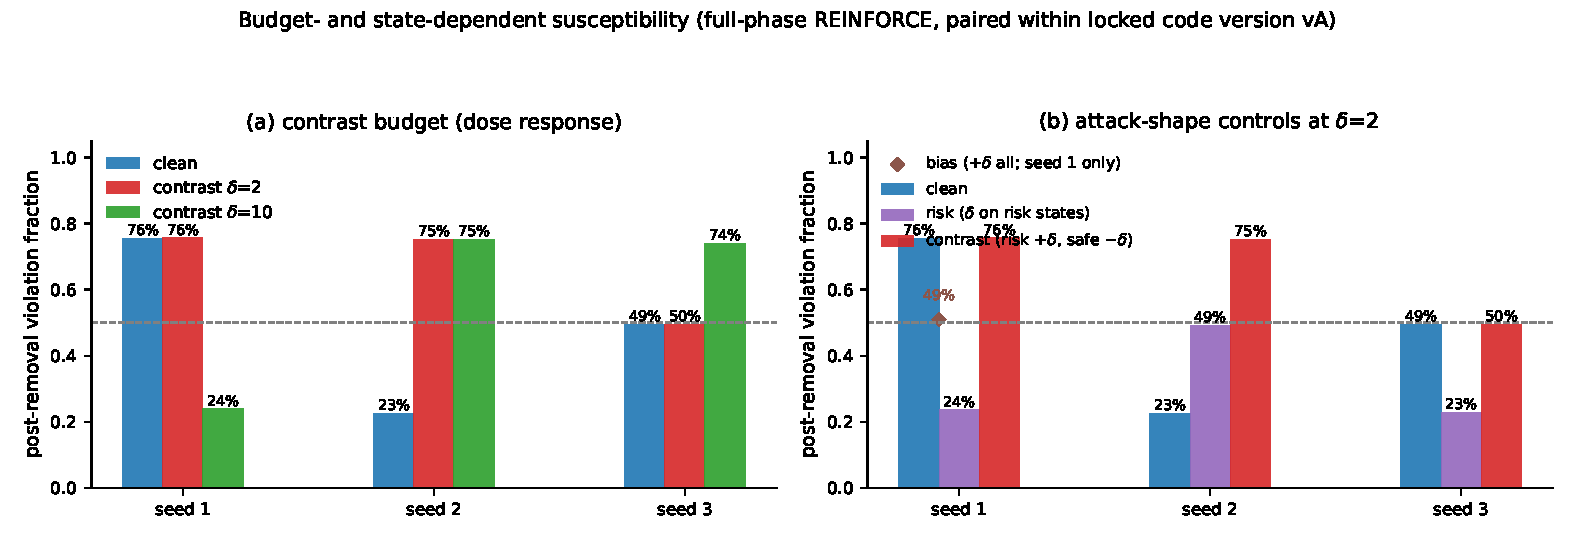
\includegraphics[width=\textwidth]{fig7_dose_response.pdf}
\caption{Budget- and state-dependent effects on the full-phase REINFORCE
protocol (paired within one locked code version).  (a) Contrast
attack dose response; (b) attack-shape negative controls at $\delta{=}2$.
The run-index-2 realization saturates at $\delta{=}2$; the run-index-3
realization requires $\delta{=}10$; the ceiling realization shows no additional damage at
either budget, and bias/risk controls are protective or strictly weaker.}
\label{fig:dose-response}
\end{figure*}

\subsection{Environment Boundary}

On a second gridworld of the same third-party suite (surveillance, $N{=}6$,
$R{=}3$), a clean reproduction again satisfied the authors' lifecycle
ordering: shield retained
$0/0$, smooth $0.129$, sudden $0.246$, and no-shield $0.252$ (retained $<$
smooth $\ll$ sudden $\le$ no-shield).  The fixed contrast attack at
$\delta{=}2$ raised post-removal violations in one of three independent paired
runs ($0.000 \rightarrow 0.272$, McNemar exact $p=2.6\times10^{-82}$) and was
protective in the other two ($0.267 \rightarrow 0.000$,
$p=8.4\times10^{-81}$; $0.135 \rightarrow 0.038$,
$p=1.3\times10^{-15}$).  The lifecycle ordering extended to the second
environment, whereas the exploit effect remained environment- and
realization-dependent.

\subsection{Opportunity-Region Cross-Tabulation}

Figure~\ref{fig:two-by-two} plots the coarse two-by-two
cross-tabulation summarized in Section~\ref{sec:third-party}: across 53
locked paired runs spanning both scopes, all three learner families, and
both domains, 12 of 20 runs with clean at-retirement violation below $0.5$
were positive, whereas none of 33 ceiling runs was positive.

\begin{figure*}[t]
\centering
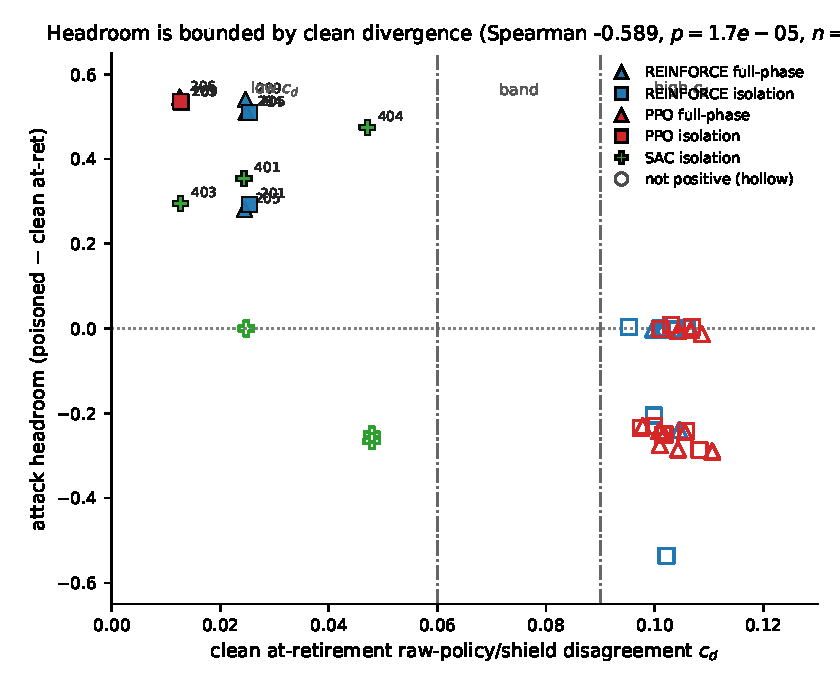
\includegraphics[width=0.72\textwidth]{fig9_mechanism_divergence.pdf}
\caption{Clean at-retirement raw-policy/shield disagreement marks an
opportunity region across the obstacle corpus (both scopes, all three learner
families).  Each point is one paired clean/poisoned run; filled markers meet
the positive-outcome rule, and hollow markers do not.
Filled markers all have clean disagreement $\le0.047$; the dashed lines mark
the fixed low/high disagreement bands ($<0.06$ and $\ge0.09$).  No
high-disagreement run is positive, while seven of 18 low-disagreement runs are
non-positive.}
\label{fig:mechanism}
\end{figure*}

\begin{figure*}[t]
\centering

\includegraphics[width=\textwidth]{fig8_2x2_susceptibility.pdf}
\caption{Two-by-two opportunity-region cross-tabulation across all locked
paired runs (both scopes, all three learner families, both domains).  Each
point is one paired clean/poisoned run; filled markers meet the positive rule
(poisoned at-retirement at least $0.15$ above clean at retirement with paired
McNemar exact $p<0.01$), hollow markers do not.  The dashed rule line is
$y=x+0.15$ and the vertical dashed line marks the clean at-retirement $0.5$
boundary: positive outcomes concentrate below $0.5$, and no ceiling run is
positive.}
\label{fig:two-by-two}
\end{figure*}

\subsection{Family-Stratified Counts and Band Chronology}

Family-stratified counts clarify the AUC reported in
Section~\ref{sec:third-party}.  REINFORCE had seven positive low-band runs and
13 non-positive high-band runs.  PPO had one positive low-band run and 19
non-positive high-band runs.  All ten SAC runs were low-band, with three
positive and seven non-positive outcomes.

The protocol chronology bounds the statistical interpretation.  The
$0.06/0.09$ bands were fixed after analysis of 46 existing obstacle rows and
before four SAC extension pairs with run indices 407--410.  All four
extensions were low-band and non-positive.  They strengthened the
non-sufficiency result without prospectively testing high-disagreement
exclusion.  The marker is also obstacle-scoped: two protective runs in the
second environment had clean disagreement $0.476$ and $0.157$ despite clean
violation below $0.5$.


\section{LifecycleGate Semantic Benchmarks}
\label{sec:appendix-benchmarks}

This appendix contains the low-dimensional semantic benchmarks that
distinguish current-action filtering from update admission.  They instantiate
the certificate semantics of Section~\ref{sec:gate} rather than the
authority-transition attack evaluated in Section~\ref{sec:study}.

\subsection{Setup}

We instantiated the linear system of Appendix~\ref{sec:appendix-lift} with
$\lambda=1.2$,
$u_{\max}=0.2$, and $S=[-1,1]$.  FDI induced the ambiguity set
$X_{\mathcal A}(h)=[-\rho,\rho]$.  The common certified kernel for invariant
certificate $I=S$ is
\begin{equation}
    K(\rho)=[-u_{\max},u_{\max}]\cap[-1+\lambda\rho,1-\lambda\rho].
\end{equation}
The kernel is nonempty exactly when $\lambda\rho\le 1$.

\subsection{Learning-Freeze Frontier}

The frontier occurs at $\rho=1/\lambda=0.833$. Table~\ref{tab:frontier} shows the exact kernel values for representative ambiguity radii.

\begin{table}[t]
\centering
\caption{Certified kernel for the one-dimensional ambiguity set.}
\label{tab:frontier}
\begin{tabular}{cccc}
\toprule
$\rho$ & $\lambda\rho$ & $K(\rho)$ & Gate \\
\midrule
0.600 & 0.720 & $[-0.200,0.200]$ & allow \\
0.800 & 0.960 & $[-0.040,0.040]$ & constrain \\
0.833 & 1.000 & $\{0\}$ & boundary \\
0.900 & 1.080 & $\emptyset$ & freeze/reject \\
1.000 & 1.200 & $\emptyset$ & freeze/reject \\
\bottomrule
\end{tabular}
\end{table}

At $\rho=0.9$, states $+0.9$ and $-0.9$ are individually controllable when
their sign is trusted.  Their safe intervals are $[-0.2,-0.08]$ and
$[0.08,0.2]$, respectively.  The empty intersection prevents a common
history-dependent action from being certified.

\subsection{Trusted Anchors and Learning-Aware FDI}

A trusted state anchor can restore learning by shrinking the plausible-state
set.  At $\rho=0.9$, a trusted sign anchor reduces the set to $[0,0.9]$ or
$[-0.9,0]$.  The corresponding kernels, $[-0.2,-0.08]$ and $[0.08,0.2]$,
are nonempty.

Learning-aware FDI creates the complementary failure mode.  For a candidate
action $u=0.1$, the gate allows the update at $\rho=0.6$, projects it to
$0.04$ at $\rho=0.8$, and rejects it at $\rho=0.9$.  The attacked history
therefore determines whether the same candidate is allowed, constrained, or
rejected.

\subsection{Lifecycle Benchmark Results}

We compared five mechanisms over five update steps: an ungated learner, a
nominal action filter, a robust action filter, always-freeze, and LifecycleGate
with projection.  The one-dimensional benchmark used the system above.  The
linear tank benchmark used the level-deviation model
\begin{equation}
    x_{t+1}=Ax_t+Bu_t,
    \quad
    A=\begin{bmatrix}1.08&0.04\\0.02&1.03\end{bmatrix},
    \quad
    B=\begin{bmatrix}1\\0.1\end{bmatrix},
\end{equation}
with $|u_t|\le 0.15$ and $x_t\in[-1,1]^2$. The nonlinear tank benchmark uses square-root inter-tank and drain flows,
\begin{equation}
\begin{aligned}
h_{1,t+1} &= h_{1,t}+\Delta t(q_0+u_t-q_{12}(h_t)-d_1(h_{1,t})),\\
h_{2,t+1} &= h_{2,t}+\Delta t(q_{12}(h_t)-d_2(h_{2,t})),
\end{aligned}
\end{equation}
where $q_{12}$ and $d_i$ are square-root flow terms.  Its interval observer
returned a box around the nominal attacked history.  The one-step kernel was
computed over a grid within that box.  In all benchmarks, learning-aware FDI
pushed the learner toward a larger positive action parameter.

\begin{figure*}[t]
\centering
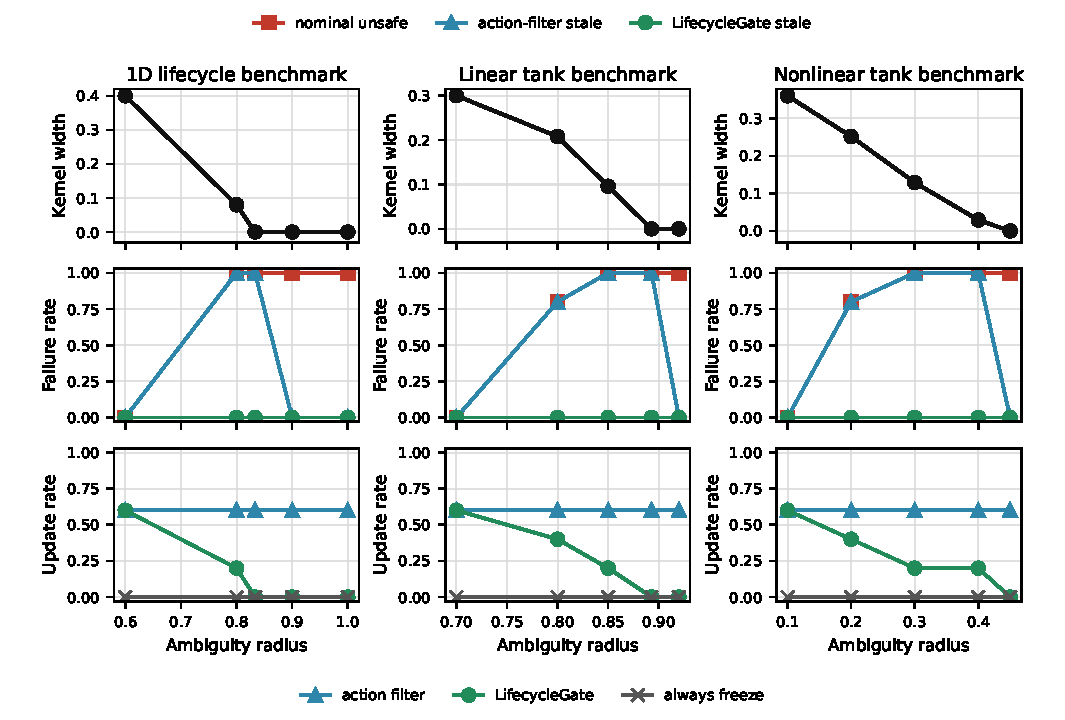
\includegraphics[width=\textwidth]{lifecycle_gate_summary.pdf}
\caption{Lifecycle-gate benchmark results.  Increasing ambiguity shrinks the
certified kernels of the one-dimensional, linear-tank, and nonlinear-tank
models.  LifecycleGate constrains or freezes updates when action-only filters
would leave the updated policy outside the kernel.}
\label{fig:lifecycle-benchmarks}
\end{figure*}

Figure~\ref{fig:lifecycle-benchmarks} separates current-action filtering from
update certification.  At $\rho=0.8$, the nominal filter had unsafe certified
rate $1.0$.  The robust action filter had stale-policy rate $1.0$ because the
learner parameter left $K(\rho)$ after action projection.  LifecycleGate had
zero unsafe or stale operation and retained one of five updates.  At
$\rho=0.9$, the kernel was empty and LifecycleGate froze learning.

The linear tank benchmark reproduced the same pattern.  At $\rho=0.8$,
nominal filtering had unsafe certified rate $0.8$, and robust action filtering
had stale-policy rate $0.8$.  LifecycleGate kept both rates at zero and allowed
two of five updates.  It allowed one constrained update at $\rho=0.85$ and
froze at the empty-kernel point $\rho=0.92$.

The nonlinear tank benchmark preserved the separation with kernels computed
from sampled nonlinear dynamics.  At $\rho=0.2$, nominal filtering was unsafe
in four of five steps, and robust filtering was stale in four.  LifecycleGate
kept both rates at zero while allowing two constrained updates.  At
$\rho=0.45$, the interval-observer box admitted no common safe action and
LifecycleGate froze the update.

\subsection{Parameter-Level Update Gate}

We also instantiated the gate at the parameter level for linear policy
$u=kz+b$.  Each future attacked observation $z$ induced a safe-action kernel
over ambiguity interval $[z-\rho,z+\rho]$.  Requiring $kz+b$ to lie in every
kernel produced linear halfspace constraints on $(k,b)$.  The parameter gate
projected poisoned candidates onto this certified set.

\begin{figure}[t]
\centering
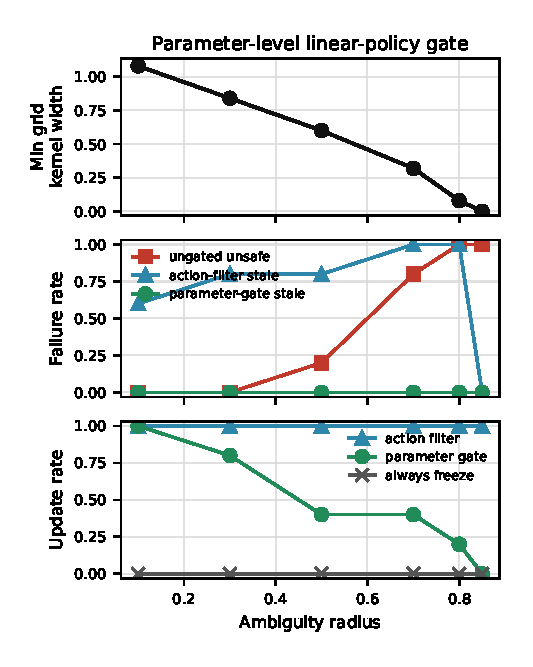
\includegraphics[width=\columnwidth]{parameter_gate_summary.pdf}
\caption{Parameter-level gate for linear policy $u=kz+b$.  Current-action
filtering leaves the future action map stale, whereas projection onto the
certified halfspace set constrains the full update.}
\label{fig:parameter-gate}
\end{figure}

Figure~\ref{fig:parameter-gate} shows the parameter-level frontier.  At
$\rho=0.7$, current-action filtering had stale-policy rate $1.0$.  The
parameter gate kept the rate at zero and permitted two of five updates.  It
permitted one constrained update at $\rho=0.8$ and froze at $\rho=0.85$.
Figure~\ref{fig:matrix-parameter-gate} repeats the comparison for the matrix
parameterization.

\begin{figure}[t]
\centering
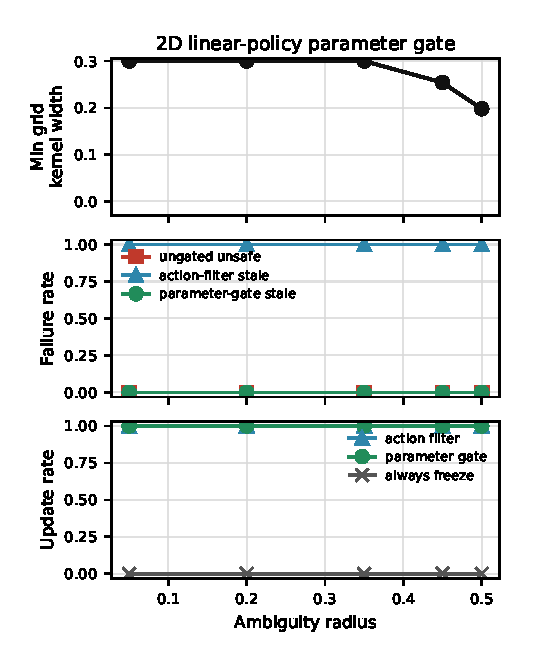
\includegraphics[width=\columnwidth]{matrix_parameter_gate_summary.pdf}
\caption{Parameter-level gate for the two-dimensional linear tank policy.  The
certified set intersects future-history halfspaces, and the gate projects the
poisoned update into that set.}
\label{fig:matrix-parameter-gate}
\end{figure}

We applied the same construction to policy $u=k_1z_1+k_2z_2+b$.  Each grid
observation induced a plausible-state box and a one-step safe-action interval.
These intervals produced halfspaces in $(k_1,k_2,b)$.  At $\rho=0.5$,
current-action filtering had stale-policy rate $1.0$.  The parameter gate kept
the rate at zero and admitted all five projected updates.

\subsection{Adaptive Attacker Stress Test}

We next allow a finite-search white-box attacker to select among poisoned
update directions.  Its objectives maximize stale-policy, unsafe-action, or
forced-freeze outcomes.  For forced freeze, the attacker also selects the
budget-feasible ambiguity radius that most reduces the certified set.

\begin{figure}[t]
\centering
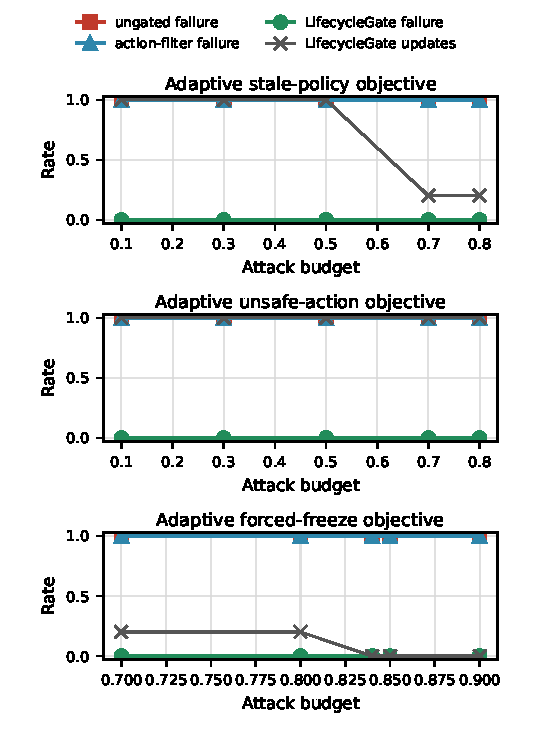
\includegraphics[width=0.98\columnwidth]{adaptive_attack_summary.pdf}
\caption{Finite-search attacker against the scalar parameter gate.  The
attacker selects update directions or ambiguity radii for three objectives.
LifecycleGate freezes when the certified kernel is empty.}
\label{fig:adaptive-attacker}
\end{figure}

Figure~\ref{fig:adaptive-attacker} preserves the lifecycle separation under
adaptive direction search.  At high ambiguity, the robust action filter
protected the applied action but left the raw policy stale.  LifecycleGate
kept unsafe, stale, and uncertified-learning rates at zero while allowing
feasible projected updates.  At $\rho=0.84$, the forced-freeze objective made
the common kernel empty.  The robust filter recorded five uncertified learner
updates, whereas LifecycleGate performed none.

\subsection{Safe-Control-Gym Cartpole Semantics}

We next instantiate the lifecycle condition in the Safe-Control-Gym cartpole
benchmark.  The official linear-quadratic regulator (LQR) is augmented with a
two-parameter linear residual learner.  The attacker injects continuous
observation FDI and optimizes a cross-entropy-method (CEM) objective over
stale-policy, unsafe-action, and forced-freeze margins.  The attacked
observation $z$ and radius $\rho$ induce the plausible box
$X_{\mathcal A}(z)=\{x:\|x-z\|_\infty\le \rho\}$.  We sample this box and
evaluate the official CasADi cartpole dynamics over an action grid to compute
$K_\Gamma(z)$.  A reference run uses the official cartpole CBF and its sampled
Lie-derivative condition.

This experiment is a direct semantic implementation of
Theorem~\ref{thm:gate} and Proposition~\ref{prop:parameter-gate}. The
future-history abstraction $\mathcal Z$ is a local grid of future attacked
observations around the current attacked observation. For each
$z'\in\mathcal Z$, the robust kernel produces an interval
$K_\Gamma(z')=[\ell_{z'},u_{z'}]$. The LQR term is fixed, while the residual
learner is linear in $(\theta_{\mathrm{gain}},\theta_{\mathrm{bias}})$, so
requiring the updated residual policy to stay inside all future kernels yields
the halfspace constraints used by LifecycleGate.

\begin{figure*}[t]
\centering
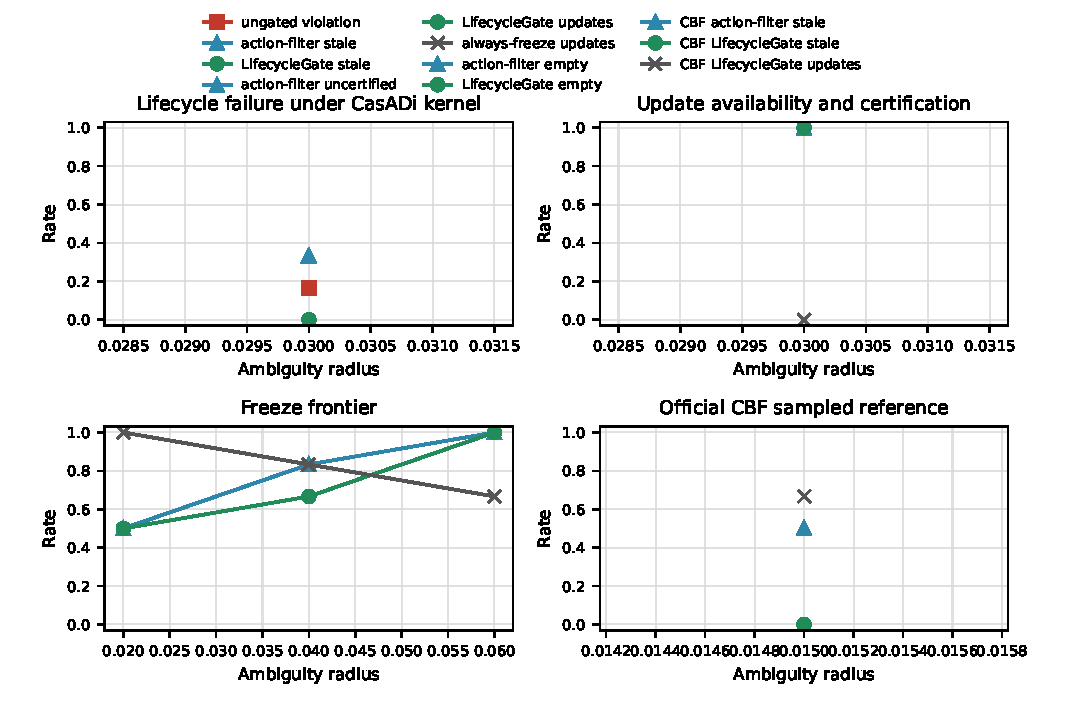
\includegraphics[width=\textwidth]{safe_control_gym_paper_mini_summary.pdf}
\caption{Safe-Control-Gym cartpole lifecycle evidence from a two-run sweep.
The panels compare the CasADi robust kernel, an Euler attack-search surrogate,
and a sampled CBF reference.  At $\rho=0.03$, LifecycleGate eliminated stale
and uncertified updates while retaining update availability.  The kernel became
empty as ambiguity increased.}
\label{fig:safe-control-gym}
\end{figure*}

Figure~\ref{fig:safe-control-gym} separates three effects.  Action filtering
removed current constraint violations without certifying the updated residual
policy.  Always-freeze avoided stale certification but admitted no learning.
LifecycleGate projected feasible poisoned updates into the future-history
halfspace set, preserving update availability before the freeze frontier.  At
larger ambiguity radii, the kernel became empty and LifecycleGate froze the
update.  These results instantiate the certificate semantics in a standard
control benchmark; the evaluation does not represent an industrial deployment.

\section{Certificate Coverage and Model Mismatch}
\label{sec:appendix-coverage}
\label{sec:coverage-appendix}

Reporting zero violations only on certificate-admitted states can be
vacuous.  We therefore lock a separate CasADi--PyBullet confusion audit before
execution.  It reconstructs the 12 clean, poisoned, commit, and freeze
snapshots from the original traces, draws 144 states from three disjoint
source seeds, performs no certificate admission, and compares horizons
20/50/100 and guard margins 0/0.001/0.003/0.005/0.01.  The primary
configuration is the pre-existing 100-step, 0.003-guard commit configuration;
the grid is characterization rather than a selector.

\begin{table*}[t]
\centering
\caption{CasADi--PyBullet coverage at the pre-existing 100-step, 0.003-guard
configuration.  Each row pools three learner snapshots over the same 144
states.}
\label{tab:coverage}
% Auto-generated by generate_tdsc_result_table.py; do not edit.
\begin{tabular}{lrrrrrr}
\toprule
Snapshot & Pairs & Physical viol. & Certified & False accept & False reject & Coverage \\
\midrule
Clean REINFORCE & 432 & 6 & 426 & 0 & 0 & 0.986 \\
Poisoned action-only & 432 & 403 & 27 & 0 & 2 & 0.062 \\
Poisoned commit & 432 & 21 & 408 & 0 & 3 & 0.944 \\
Always-freeze & 432 & 0 & 432 & 0 & 0 & 1.000 \\
\bottomrule
\end{tabular}

\end{table*}

Table~\ref{tab:coverage} evaluates 1728 snapshot--state pairs.  CasADi
certifies 1293; none violates the PyBullet state box within 100 steps.
Clean, commit, and freeze coverage is 0.986, 0.944, and 1.000.  The raw
poisoned snapshots physically violate 403/432 pairs and have certificate
coverage 0.062, so their low coverage is informative rejection rather than
vacuous evidence for a safe deployed snapshot.  Across all mechanisms the
certificate conservatively rejects five physically safe pairs.  Maximum
action-interface error and actuator saturation are zero.

The grid exposes a model-mismatch boundary.  Without a guard, poisoned
snapshots produce 1, 2, and 1 false acceptances at horizons 20, 50, and 100.
Every locked positive guard removes observed false acceptance, with increasing
false rejection as the guard grows.  The value 0.003 was the declared primary
configuration before this audit.  Zero observed false acceptance on the finite
evaluation distribution does not establish continuous-state invariance.


\section{Unified Paired Security--Availability Frontier}
\label{sec:appendix-frontier}

\begin{table*}[t]
\centering
\caption{Unified paired security--availability frontier.  Wilson 95\%
intervals are $[0,0.138]$ for every 0/24 violation count and
$[0.798,0.993]$ for poisoned raw.  Intervention is a fraction of executed
steps.  $\dagger$ denotes reward truncated at the first safety failure and
therefore not a utility comparison.}
\label{tab:unified-frontier}
% Auto-generated by generate_tdsc_frontier_artifacts.py; do not edit.
\begin{tabular}{lrrrrr}
\toprule
Mechanism & Viol./rollouts & Complete & Mean reward & Interv. & Latency med./p95 (ms) \\
\midrule
Clean REINFORCE & 0/24 & 24/24 & $-0.024$ & 0.0\% & 0.027/0.029 \\
Poisoned raw & 23/24 & 1/24 & $-0.189^\dagger$ & 0.0\% & 0.027/0.029 \\
Poisoned commit & 0/24 & 24/24 & $-0.056$ & 0.0\% & 0.026/0.029 \\
Always-freeze & 0/24 & 24/24 & $-0.023$ & 0.0\% & 0.026/0.028 \\
Permanent shield & 0/24 & 24/24 & $-0.195$ & 21.3\% & 221.925/238.216 \\
Official MPSC & 0/24 & 24/24 & $-0.457$ & 100.0\% & 59.657/76.055 \\
\bottomrule
\end{tabular}

\end{table*}


\end{document}
